% !TeX root = ./ms.tex
\documentclass[modern]{aastex62}

% Load the corTeX style definitions
% !TeX root = ./ms.tex
% All the packages
\usepackage{url}
\usepackage{amsmath}
\usepackage{mathtools}
\usepackage{amssymb}
\usepackage{natbib}
\usepackage{graphicx}
\usepackage{calc}
\usepackage{etoolbox}
\usepackage{xspace}
\usepackage[T1]{fontenc} % https://tex.stackexchange.com/a/166791
\usepackage{textcomp}
\usepackage{ifxetex}
\ifxetex
  \usepackage{fontspec}
  \defaultfontfeatures{Extension = .otf}
\fi
\usepackage{fontawesome}
\usepackage{listings}
\usepackage{nicefrac}
\usepackage{booktabs}
\usepackage{longtable}

% References to text content
\newcommand{\documentname}{\textsl{article}}
\newcommand{\figureref}[1]{\ref{fig:#1}}
\newcommand{\Figure}[1]{Figure~\figureref{#1}}
\newcommand{\figurelabel}[1]{\label{fig:#1}}
\renewcommand{\eqref}[1]{\ref{eq:#1}}
\newcommand{\Eq}[1]{Equation~(\eqref{#1})}
\newcommand{\eq}[1]{\Eq{#1}}
\newcommand{\eqalt}[1]{Equation~\eqref{#1}}

% Add code, proof, and animation hyperlinks
\definecolor{linkcolor}{rgb}{0.1216,0.4667,0.7059}
\definecolor{testpasscolor}{rgb}{0.13333333,0.5254902,0.22745098}
\definecolor{testmissingcolor}{rgb}{1.0,0.88,0.30}
\definecolor{testfailcolor}{rgb}{0.79607843,0.14117647,0.19215686}
\newcommand{\codeicon}{{\color{linkcolor}\faCloudDownload}}
\newcommand{\testmissingicon}{{\color{testmissingcolor}\faQuestion}}
\newcommand{\testpassicon}{{\color{testpasscolor}\faCheck}}
\newcommand{\testfailicon}{{\color{testfailcolor}\faTimes}}
\input{gitlinks}

% Define a proof environment for open source equation proofs
\newtagform{eqtag}[]{(}{)}
\newcommand{\currentlabel}{None}
\newenvironment{proof}[1]{%
  \ifstrempty{#1}{%
    \renewtagform{eqtag}[]{\raisebox{-0.1em}{{\testmissingicon}}\,(}{)}%
  }{%
    \renewtagform{eqtag}[]{\prooflink{#1}\,(}{)}%
  }%
  \usetagform{eqtag}%
  \renewcommand{\currentlabel}{#1}
  \align%
}{%
  \endalign%
  \renewtagform{eqtag}[]{(}{)}%
  \usetagform{eqtag}%
  \message{<<<\currentlabel: \theequation>>>}%
}

% Define the `oscaption` command for open source figure captions
\newcommand{\oscaption}[2]{\caption{#2 \codelink{#1}}}

% Code examples
\definecolor{codegreen}{rgb}{0,0.6,0}
\definecolor{codegray}{rgb}{0.5,0.5,0.5}
\definecolor{codepurple}{rgb}{0.58,0,0.82}
\definecolor{backcolour}{rgb}{0.95,0.95,0.95}
\lstdefinestyle{mystyle}{
  backgroundcolor=\color{backcolour},
  commentstyle=\color{codegreen},
  keywordstyle=\color{magenta},
  numberstyle=\tiny\color{codegray},
  stringstyle=\color{codepurple},
  basicstyle=\small\ttfamily,
  breakatwhitespace=false,
  breaklines=true,
  captionpos=b,
  keepspaces=true,
  numbers=left,
  numbersep=5pt,
  showspaces=false,
  showstringspaces=false,
  showtabs=false,
  tabsize=2,
  aboveskip=1em,
  belowskip=1em,
  keywords=[2]{map},
  keywordstyle=[2]{\color{black!80!black}},
  upquote=true
}
\lstset{style=mystyle}

% Typography obsessions
\setlength{\parindent}{3.0ex}
\renewcommand\quad{\hskip\fontdimen3\font}

% https://tex.stackexchange.com/a/184474
\usepackage{stackengine,scalerel}
\def\lnlam{\ThisStyle{\ensurestackMath{\stackon[-2.4\LMpt]{%
        \SavedStyle\lambda}{\kern-.5pt\kern\LMpt\rule{1\LMex}{.25pt+.15\LMpt}}}}}


% Load custom style
% Packages
\usepackage{xifthen}
\usepackage{stackengine}
\usepackage{tabstackengine}
\usepackage{array}
\usepackage{upgreek}
\usepackage[bbgreekl]{mathbbol}
\usepackage{afterpage}
\usepackage[bb=boondox]{mathalpha}

% Shorthand for this paper
\newcommand{\starry}{\textsf{starry}\xspace}
\newcommand{\cpp}{\textsf{C++}\xspace}
\newcommand{\theano}{\textsf{theano}\xspace}
\newcommand{\pymcthree}{\textsf{pymc3}\xspace}
\newcommand{\starryprocess}{\textsf{starry\_process}\xspace}
\newcommand{\Python}{\textsf{Python}\xspace}
\newcommand{\xxx}[1]{{\color{red}#1}}
\newcommand{\quadquad}{\quad\quad\quad\quad}

% Misc. macros
\newcommand{\LMAX}{15\xspace}

% Integrals
\newcommand{\dd}{\ensuremath{\text{d}}}

% Special functions
\newcommand{\sgn}{{\text{sgn}}}
\newcommand{\atantwo}{{\text{arctan2}}}

% Cartesian unit vectors
\newcommand{\xhat}{\ensuremath{\pmb{\hat{x}}}\xspace}
\newcommand{\yhat}{\ensuremath{\pmb{\hat{y}}}\xspace}
\newcommand{\zhat}{\ensuremath{\pmb{\hat{z}}}\xspace}

% Other
\DeclarePairedDelimiter\ceil{\lceil}{\rceil}
\DeclarePairedDelimiter\floor{\lfloor}{\rfloor}

% Inverse diagonal dots
\makeatletter
\def\Ddots{\mathinner{\mkern1mu\raise\p@
        \vbox{\kern7\p@\hbox{.}}\mkern2mu
        \raise4\p@\hbox{.}\mkern2mu\raise7\p@\hbox{.}\mkern1mu}}
\makeatother

% Imaginary unit
\DeclareFontFamily{U}{mathc}{}
\DeclareFontShape{U}{mathc}{m}{it}{<->s*[1.03] mathc10}{}
\DeclareMathAlphabet{\mathscr}{U}{mathc}{m}{it}
\DeclareMathOperator{\imag}{\mathscr{i}}


% Bibliography
\bibliographystyle{aasjournal}

\usepackage{etoolbox}
\makeatletter % we need to patch \env@cases that has @ in its name
\patchcmd{\env@cases}{\quad}{\qquad\qquad}{}{}
\makeatother

\usepackage{enumitem}

% Begin!
\begin{document}

% Title
\title{%
    \textbf{
        Mapping stellar surfaces\\
        I: Degeneracies in the light curve problem
    }
}

% Author list
\author[0000-0002-0296-3826]{Rodrigo Luger}\altaffiliation{Flatiron Fellow}
\email{rluger@flatironinstitute.org}
\affil{Center~for~Computational~Astrophysics,~Flatiron~Institute,~New~York,~NY}
\affil{Virtual~Planetary~Laboratory, University~of~Washington, Seattle, WA}
%
\author[0000-0002-9328-5652]{Daniel Foreman-Mackey}
\affil{Center~for~Computational~Astrophysics,~Flatiron~Institute,~New~York,~NY}
%
\author[0000-0002-3385-8391]{Christina Hedges}
\affil{Bay~Area~Environmental~Research~Institute,~P.O.~Box~25,~Moffett~Field,~CA~94035,~USA}
\affil{NASA~Ames~Research~Center,~Moffett~Field,~CA}
%

\keywords{time series analysis --- light curves --- stellar surfaces --- starspots}

\features{open-source figures \codeicon; equation unit tests: \input{tests/tally}}

\begin{abstract}
    \xxx{Abstract here.}
\end{abstract}

\section{Introduction}
\label{sec:intro}

The advent of space-based precision photometry with missions such as
\emph{Kepler} \citep{Borucki2010} and \emph{TESS} \citep{Ricker2015}
has led to a renewed interest in the modeling of stellar light curves,
and, in particular, in understanding what these light curves can tell
us about the surfaces of stars across the HR diagram. One of the dominant
sources of stellar light curve variability is the modulation caused
by starspots rotating in and out of view.
Dark spots arise due to the suppression of convection in regions of
intense magnetic field, resulting in a locally cooler (and hence darker)
photosphere. Bright spots can similarly
arise in the photosphere as faculae or in the chromosphere as plages, and
are also magnetically driven \citep[e.g.,][]{Berdyugina2005}.
%
Constraining the sizes,
contrasts, locations, and number of spots on stars can therefore reveal
information about stellar magnetic activity, stellar interior structure,
and how these quantities vary across spectral type and over time.
A detailed understanding of the stellar surface is also crucial to
mitigating systematics in the radial velocity search for exoplanets
\citep[e.g.,][]{Lanza2011} and in the spectroscopic characterization of their
atmospheres \citep[e.g.,][]{Rackham2018}.

To date, most studies aimed at inferring stellar surface
properties from light curves follow one of two broad approaches. The
first is to model the stellar surface as a collection of one or more
discrete, circular, uniform contrast dark or bright spots on a uniform
intensity photosphere.
The advantage of this approach is that
the light curve can be computed efficiently and in some cases even
analytically \citep[e.g.,][]{Davenport2015,Morris2017,Morris2020b}.
%
The second approach is to discretize the surface at some resolution
and compute the emergent flux as a weighted sum of the visible pixel intensities.
This approach is more flexible, since it is not limited to surfaces
composed of distinct circular spots \citep[e.g.,][]{Harmon2000,Roettenbacher2017}.
%
Both approaches rely on an explicit \emph{forward model}, a prescription for
how to generate data given a set of parameters. In most cases, however, we are interested
in the inverse problem: constraining the parameters given data.
%
Unfortunately, the inverse problem is not only difficult---as it requires
a large number of forward model evaluations to find the parameter values
that are most consistent with the
data---but also formally \emph{ill-posed}.
%
While the mapping from a stellar surface to a light curve (the forward
problem) is unique, the mapping from a light curve to a surface
(the inverse problem) is not:
given any light curve, there exist an infinite number of surfaces that
could have generated it. These degeneracies are illustrated in
Figure~\ref{fig:degeneracies}, where six synthetic stellar surfaces
are shown (rows) at twelve different phases (columns), all at an
inclination $I=60^\circ$. Each surface
consists of a different number of dark spots on a brighter, heterogeneous
background.

\begin{figure}[t!]
    \begin{centering}
        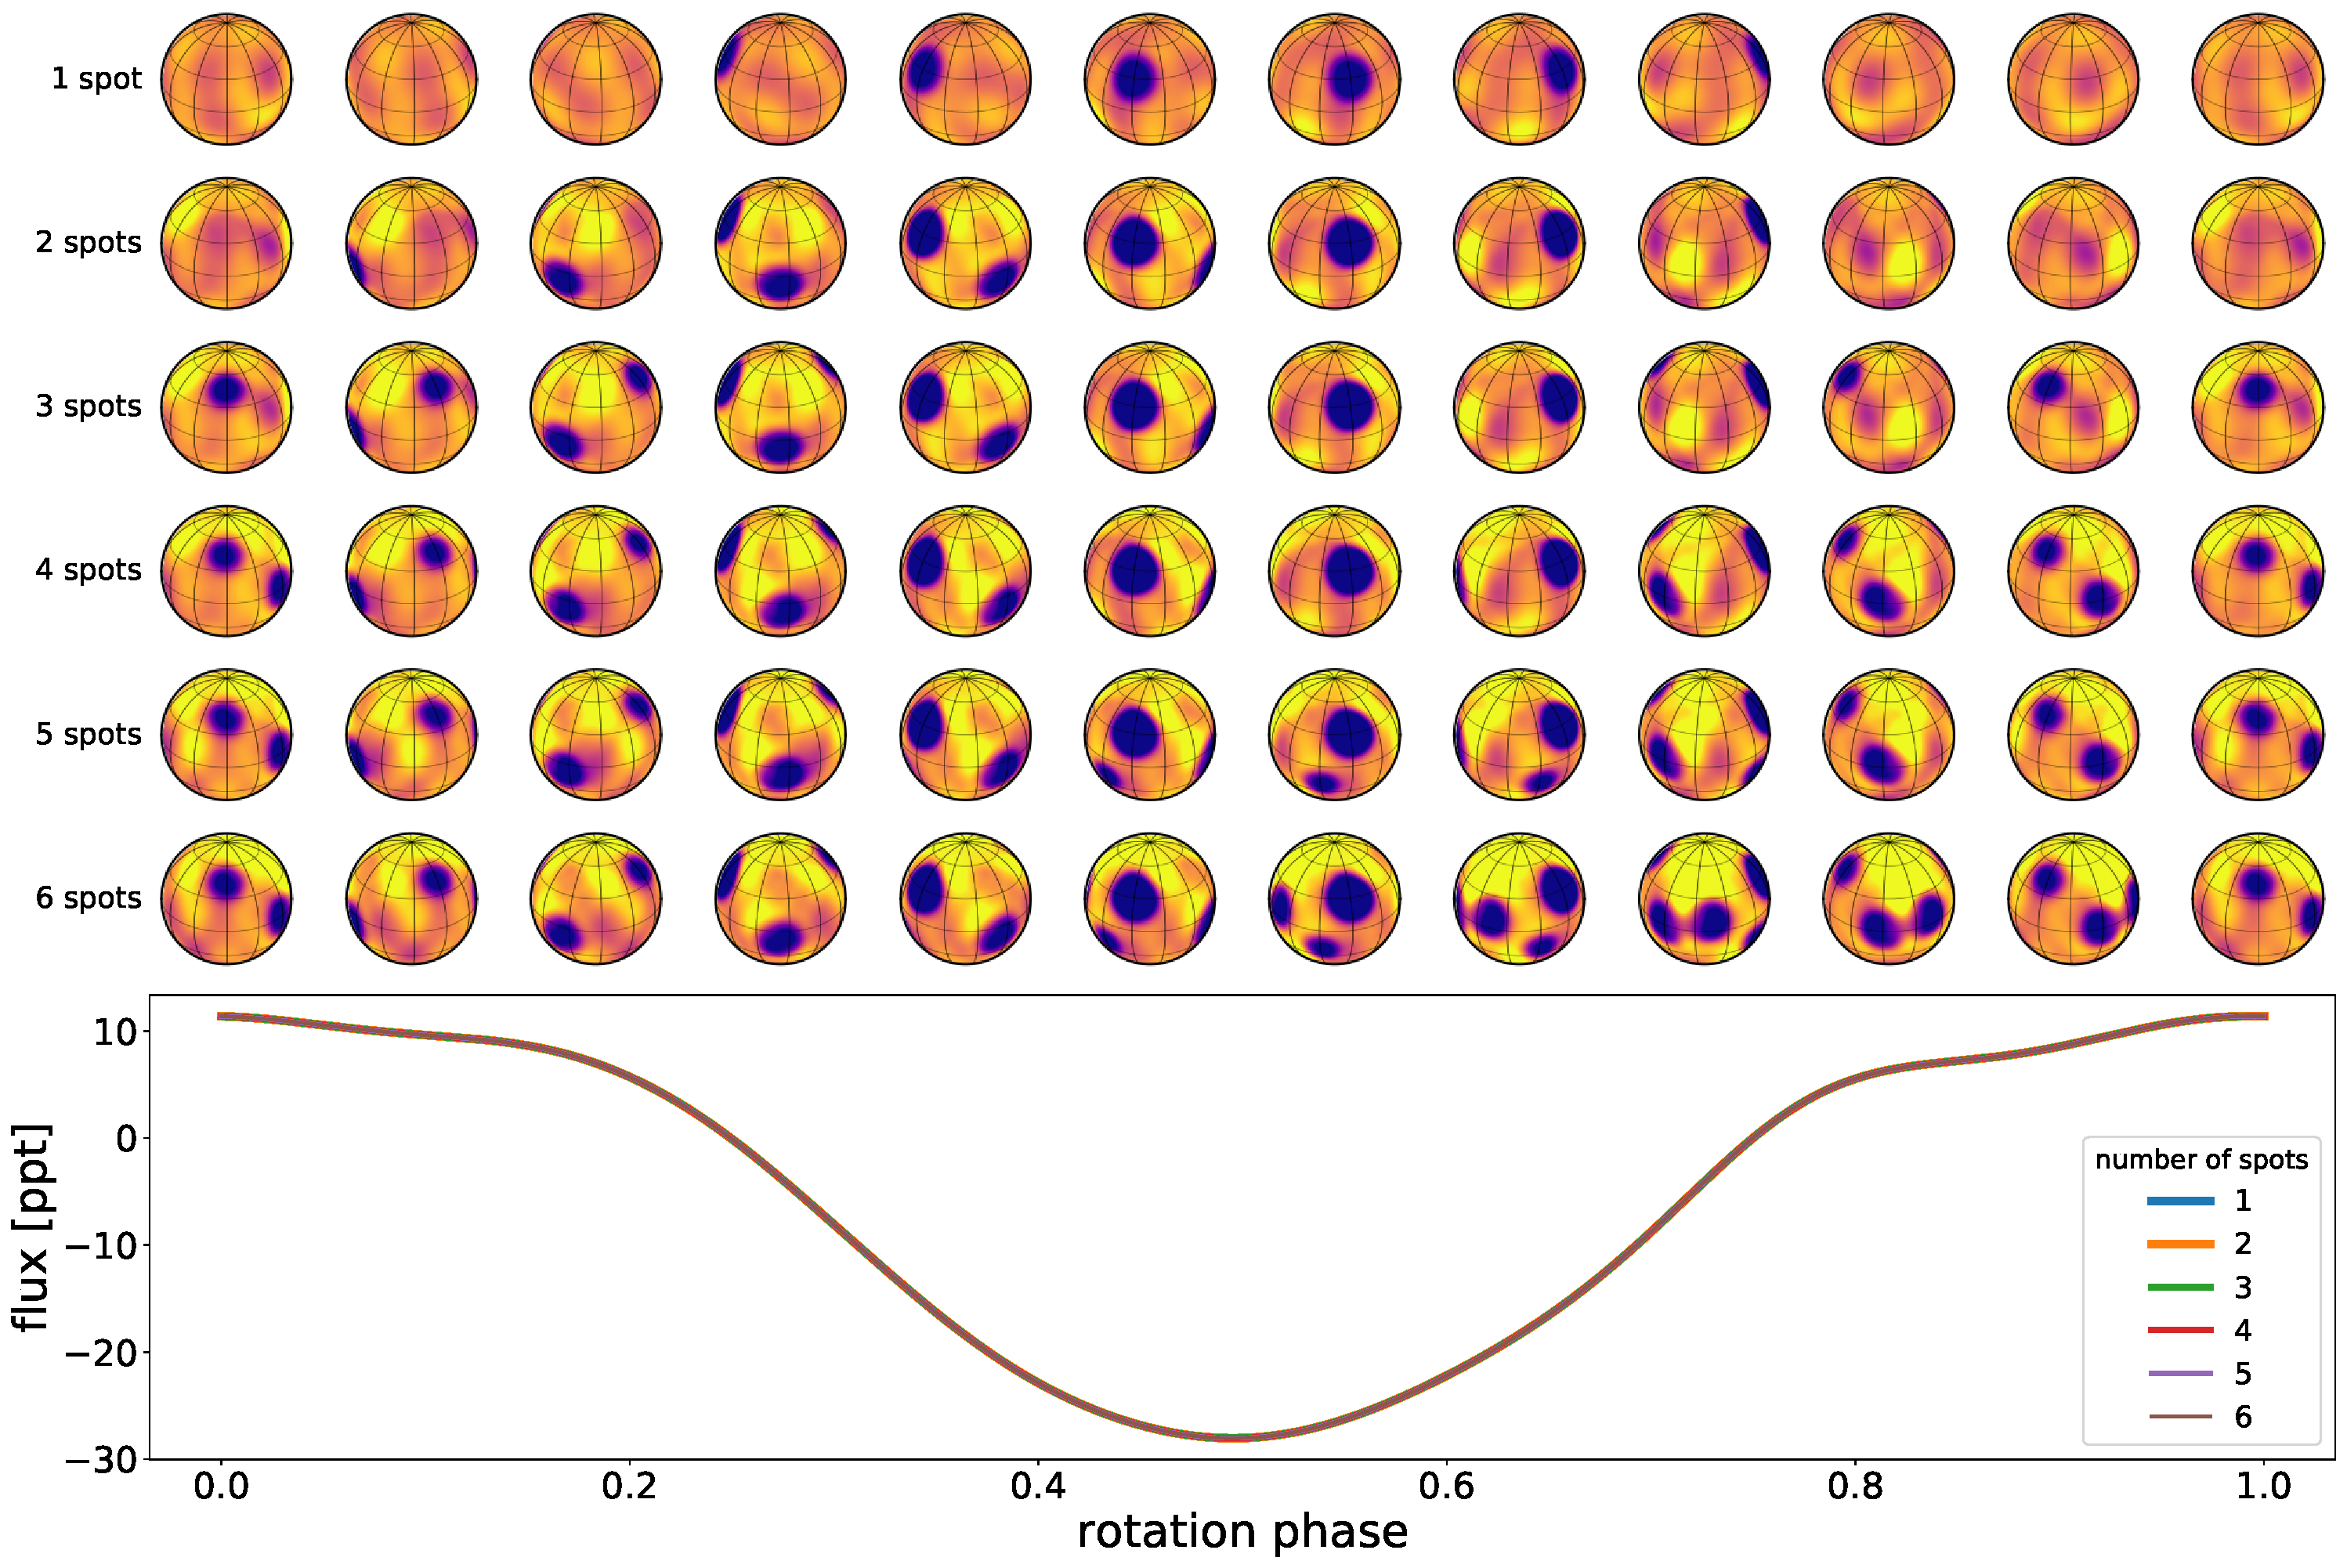
\includegraphics[width=\linewidth]{figures/degeneracies.pdf}
        \oscaption{degeneracies}{%
            The fundamental limitations of the mapping problem. Each row
            corresponds to a stellar surface with a different number of
            dark spots seen at various phases at an inclination $I=60^\circ$;
            all images are shown on the same color scale.
            The bottom panel shows the light curves of each of these stars.
            All six light curves are indistinguishable from each other, even
            at infinite signal to noise. See text for details.
            \label{fig:degeneracies}
        }
    \end{centering}
\end{figure}

While the stellar surfaces are all distinct, containing between one (top)
and six (bottom) large dark spots,
\textbf{their rotational light curves are identical}
(lower panel). This is true even at infinite signal to
noise: the mapping from a stellar surface
to its rotational light curve is so degenerate that there exist an infinite number of solutions
to the inverse problem. This fact has been pointed out recently in different contexts
\citep[e.g.,][]{Cowan2013,Luger2019,Basri2020}, but it dates back at least to
\citet{Russell1906}, who demonstrated it by expanding the surface
intensity of a celestial body in terms of spherical harmonics.
(see Figure~\ref{fig:ylms}). \citet{Russell1906} showed
that many of the modes comprising the intensity profile of a spherical
object are in the \emph{null space}, the set of surface features that have identically
zero effect on the light curve. In fact,
the \emph{vast majority} of the modes are in the null space for rotational
light curves of stars (\S\ref{sec:nullspace}). This is what allows us to construct pathological
scenarios like that shown in Figure~\ref{fig:degeneracies}, where the light curve
could be explained by any number of spots atop a heterogeneous bright background.

\begin{figure}[t!]
    \begin{centering}
        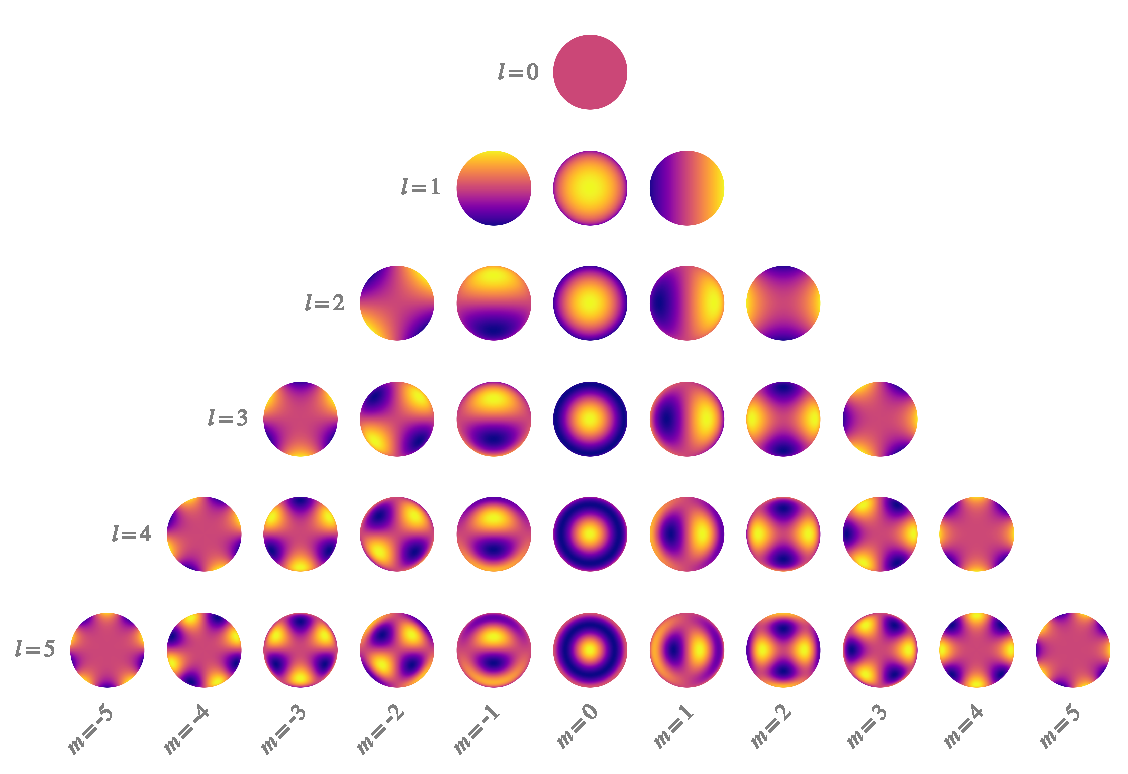
\includegraphics[width=\linewidth]{figures/ylms.pdf}
        \oscaption{ylms}{%
            The real spherical harmonics in the polar frame up to
            $l = 5$, where dark colors correspond to negative intensity
            and bright colors to positive intensity.
            Rows correspond to the degree $l$ and columns to
            the order $m$. The set of all spherical harmonics forms a
            complete, orthogonal basis on the sphere.
            \label{fig:ylms}
        }
    \end{centering}
\end{figure}

Stellar mapping studies tackle these degeneracies in different ways, but
it usually comes down to a choice of prior: when the data is not
sufficiently informative, prior assumptions are needed to discriminate
between competing solutions. In discrete spot models like the ones
discussed above, the degeneracy-breaking prior is (typically) the assumption that the
spots must be circular, have uniform contrast, and sit atop an otherwise
uniform photosphere. In gridded stellar surface models, it is common to
assume a regularization prior such as the maximum entropy penalty
\citep[e.g.,][]{Vogt1987}, which typically favors solutions with the fewest
number of dark pixels (usually referred to as the ``simplest'' solution).

While these assumptions may be approximately valid in some cases, it is
important to bear in mind that because of the light curve degeneracies discussed above,
\textbf{most of the information about the stellar surface usually comes from the prior},
so it is very important to get the
prior right. In general, sunspots are not circular and do not have uniform
contrast throughout; nor do spots always arrange themselves in the highest
entropy configuration. The amount of bias introduced by these assumptions
will in general vary, but in principle it could be quite significant.

% Add to this photometric noise, the generally unknown stellar inclination,
% the poorly constrained limb darkening parameters, and you get ... a mess.

% Fortunately, although individual light curves are not very constraining,
% we have \emph{a lot of them} thanks to missions like \emph{Kepler} and \emph{TESS}.
% In this paper, we will thoroughly explore the power of ensemble analyses
% in breaking the degeneracies inherent to the light curve mapping problem.
% By jointly analyzing the light curves of many stars, we will show that it
% is often possible to uniquely constrain statistical properties about their
% surfaces. This idea was recently explored to some extent
% in \citet{Morris2020}, who used ensemble analyses to derive constraints on
% spot coverage areas as a function of stellar age (see \S\ref{sec:other-work}).

\xxx{In this paper...}

\section{The null space}
\label{sec:nullspace}

\subsection{Rank of the flux operator}
%
In general, inferring the properties of a stellar surface from its light curve is not
only difficult, but \emph{formally impossible}. To understand why, consider
an expansion of the stellar surface intensity in the spherical
harmonic basis out to arbitrary order (see Figure~\ref{fig:ylms}).
Assuming (for the moment) that the
star rotates about an axis that points up along the page, the observed
light curve may be expressed as a weighted sum of the disk-integrated intensity
of each of the spherical harmonics as they rotate about that same axis.
However, not all spherical harmonics will contribute to the full light curve,
as many (in fact, most) of the spherical harmonics are perfectly antisymmetric
about the equator. This is the case for
the $l = 1$, $m = -1$ harmonic, which integrates to zero regardless of
the phase at which it is viewed. The same is true, in fact, for all other harmonics
of order $m = -1$ and (perhaps less obviously) for all harmonics with odd
$l = 3, 5, 7, ...$ Furthermore, there exist many linear combinations of
spherical harmonics that similarly integrate to zero at all rotational
phases. Together, these modes constitute the \emph{null space} of the problem:
the set of modes on the surface that do not contribute to the observed
light curve and therefore cannot be probed from photometry.

For rotational light curves,
the vast majority of the surface modes lie at least partly in the null
space. To show this, we will make use of the fact that we can express
the vector of $K$ observed fluxes $\mathbf{f}$ (i.e., the light curve)
as a purely linear operation on the vector of $N$
spherical harmonic coefficients $\mathbf{y}$ \citep{Luger2019}:
%
\begin{align}
    \label{eq:fAy}
    \mathbf{f} = \mathbf{A} \, \mathbf{y}
    \quad,
\end{align}
%
where $\mathbf{A}$ is the $(K \times N)$ \emph{design matrix} of the transformation, whose columns
describe how each of the $N$ components in the spherical harmonic basis contribute
to each of the $K$ points in the light curve.%
\footnote{%
    For rotational light curves, the rows of $\mathbf{A}$ are given by the
    quantity $\mathbf{r}^\top \mathbf{A}_1 \mathbf{R}$ in Equation~(18) of
    \citet{Luger2019}, where $\mathbf{r}^\top$ is a vector of disk-integrated
    intensities, $\mathbf{A}_1$ is a change of basis matrix, and $\mathbf{R}$
    is a spherical harmonic rotation matrix that depends on the stellar inclination
    and the rotational phase of the star. Refer to that paper for more details.
}
%
Even though we are explicitly choosing the spherical harmonics as the basis in which
we describe the stellar surface, Equation~(\ref{eq:fAy}) is quite general and applies to
\emph{any} basis that is linearly related to the flux. For instance, $\mathbf{y}$
could instead describe the intensities in each of the $N$ pixels of a gridded stellar
surface, in which case $\mathbf{A}$ would be the matrix of pixel visibilities that describe
how to sum each of the pixels to obtain the observed light curve.

The size of the null space is called the \emph{nullity}, and it is equal to
$N - R$, where $N$ is once again the number of coefficients describing the
stellar surface and $R$ is the \emph{rank} of the flux operator $\mathbf{A}$.
The rank $R$ is the number of linearly independent columns in $\mathbf{A}$, which
can be easily computed with any modern linear algebra package. It is equal
to the number of independent signals (or components) that can be measured given
an observation of $\mathbf{f}$.

\begin{figure}[t!]
    \begin{centering}
        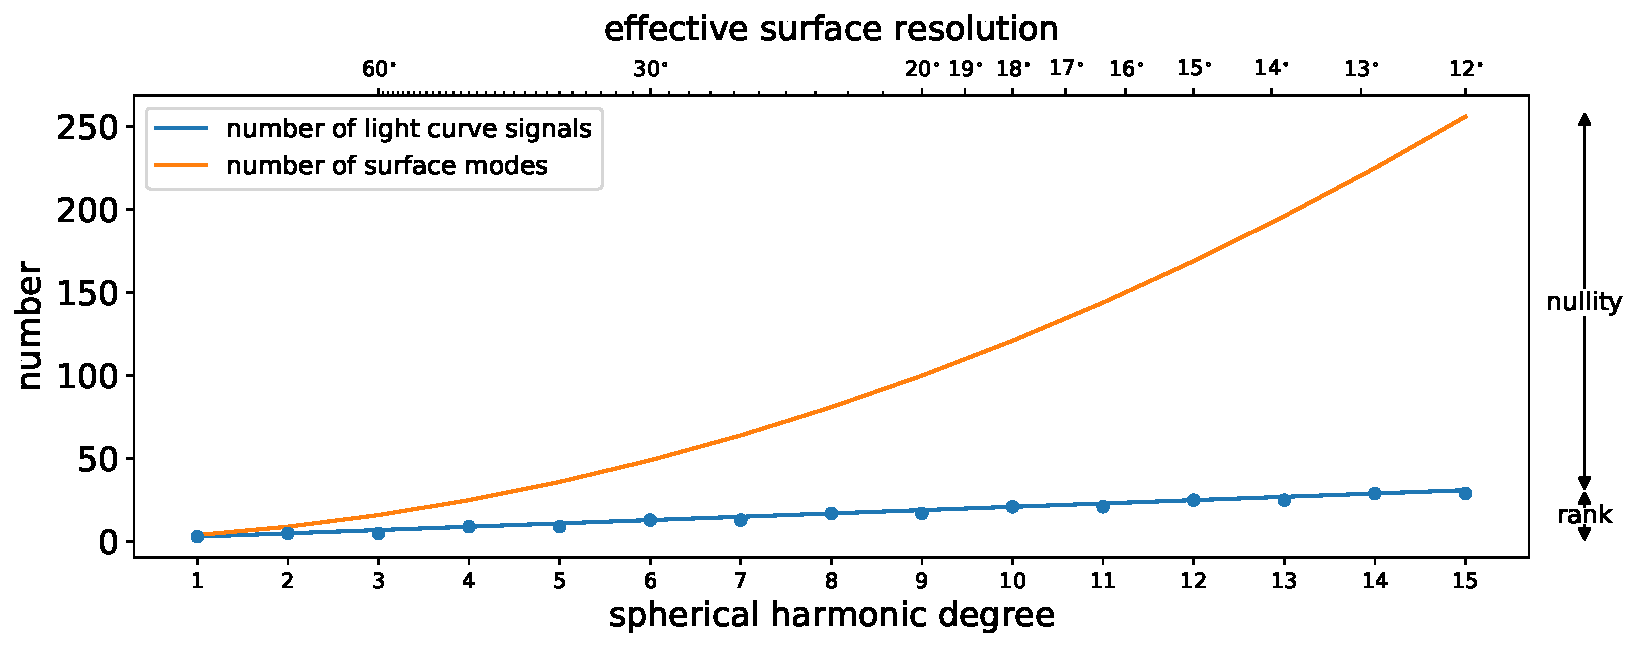
\includegraphics[width=0.65\linewidth]{figures/rank.pdf}
        \oscaption{rank}{%
            Rank and nullity of the flux operator.
            \label{fig:rank}
        }
    \end{centering}
\end{figure}

Figure~\ref{fig:rank} shows the rank and nullity of the flux operator
as a function of the resolution of the surface map (quantified as the
spherical harmonic degree $l$ of the expansion). The orange
curve is the number of spherical harmonic coefficients needed to
represent a surface map up to degree $l$, and is equal to $N = (l + 1)^2$.
The blue dots show the rank of the flux operator $\mathbf{A}$ as a function
of $l$, and the blue line is the function $R = 2l + 1$. The nullity is
simply the difference between $N$ and $R$.

The most striking feature in Figure~\ref{fig:rank} is how quickly the two
curves diverge as $l$ increases. What this means for the mapping problem
is that the number of surface modes---the total information needed to
represent a surface map at some resolution---grows much quicker than the
number of independent signals in the light curve.
%
At all but the lowest resolutions, there are always more features in the
null space than signals one can measure in the light curve, and difference
that grows \emph{quadratically} with $l$.
%
This means that although a light curve can tell us some information about
a stellar surface on very large scales, the amount of information it tells
us quickly decreases for smaller scales and all but vanishes for the smallest
surface features.

\subsection{Decomposition of the flux operator}
%
To better understand the properties of the null space of the light curve
mapping problem, let
%
us use singular value decomposition (SVD) to express
the flux operator as
%
\begin{align}
    \mathbf{A} = \mathbf{U} \, \mathbf{S} \, \mathbf{V}^\top
    \quad,
\end{align}
%
where $\mathbf{U}$ is a $(K \times K)$ orthogonal matrix,
$\mathbf{V}$ is a $(N \times N)$ orthogonal matrix,
and $\mathbf{S}$ is a $(K \times N)$ diagonal matrix.
%
The columns of $\mathbf{U}$ and the rows of $\mathbf{V}^\top$ are the left and right
\emph{singular vectors} of $\mathbf{A}$, and the entries along the
diagonal of $\mathbf{S}$ are the corresponding \emph{singular values}. If $\mathbf{A}$
has rank $R$, the first $R$ singular values will be nonzero, while the
remaining $N - R$ will be identically zero.
If we assume for definitess that $K > N$ (i.e., we have more flux observations
than surface map coefficients we're trying to constrain), we can express the
SVD matrices as
%
\begin{align}
    \mathbf{U}
     & =
    \left(
    \begin{array}{ccc|ccc}
            \mathbf{U}_{0,0}          & \cdots & \mathbf{U}_{0,R\text{-}1}          & \mathbf{U}_{0,R}          & \cdots & \mathbf{U}_{0,K\text{-}1}          \\
            \vdots                    & \cdots & \vdots                             & \vdots                    & \cdots & \vdots                             \\
            \mathbf{U}_{K\text{-}1,0} & \cdots & \mathbf{U}_{K\text{-}1,R\text{-}1} & \mathbf{U}_{K\text{-}1,R} & \cdots & \mathbf{U}_{K\text{-}1,K\text{-}1}
        \end{array}
    \right)
    \equiv
    \left(
    \begin{array}{c|c}
            \mathbf{U}_\bullet & \mathbf{U}_\circ
        \end{array}
    \right)
    %
    \\[1.5em]
    %
    \label{eq:S}
    \mathbf{S}
     & =
    \left(
    \begin{array}{ccc|ccc}
            \mathbf{S}_{0,0}\phantom{y} &                                     &                                    &                             &                                     &                                    \\
                                        & \ddots                              &                                    &                             & \mbox{\normalfont\Large\bfseries 0} &                                    \\
                                        &                                     & \mathbf{S}_{R\text{-}1,R\text{-}1} &                             &                                     &                                    \\
            \hline
                                        &                                     &                                    & \mathbf{S}_{R,R}\phantom{y} &                                     &                                    \\
                                        & \mbox{\normalfont\Large\bfseries 0} &                                    &                             & \ddots                              &                                    \\
                                        &                                     &                                    &                             &                                     & \mathbf{S}_{N\text{-}1,N\text{-}1} \\
                                        &                                     &                                    &                             &                                     &                                    \\
                                        & \mbox{\normalfont\Large\bfseries 0} &                                    &                             & \mbox{\normalfont\Large\bfseries 0} &                                    \\
                                        &                                     &                                    &                             &                                     &
        \end{array}
    \right)
    \equiv
    \left(
    \begin{array}{c|c}
            \mathbf{S}_\bullet & \mathbf{0}       \\
            \hline
            \mathbf{0}         & \mathbf{S}_\circ
        \end{array}
    \right)
    %
    \\[1.5em]
    %
    \mathbf{V}^\top
     & =
    \left(
    \begin{array}{cccccc}
            \mathbf{V}_{0,0}^\top          & \cdots & \mathbf{V}_{0,N\text{-}1}^\top          \\
            \vdots                         & \cdots & \vdots                                  \\
            \mathbf{V}_{R\text{-}1,0}^\top & \cdots & \mathbf{V}_{R\text{-}1,N\text{-}1}^\top \\[0.5em]
            \hline                                                                            \\[-0.85em]
            \mathbf{V}_{R,0}^\top          & \cdots & \mathbf{V}_{R,N\text{-}1}^\top          \\
            \vdots                         & \cdots & \vdots                                  \\
            \mathbf{V}_{N\text{-}1,0}^\top & \cdots & \mathbf{V}_{N\text{-}1,N\text{-}1}^\top
        \end{array}
    \right)
    \equiv
    \left(
    \begin{array}{cc}
            \mathbf{V}_\bullet^\top \\
            \hline
            \mathbf{V}_\circ^\top
        \end{array}
    \right)
\end{align}
%
where
$\mathbf{U}_\bullet$ is $(K \times R)$,
$\mathbf{U}_\circ$ is $(K \times K - R)$,
$\mathbf{S}_\bullet$ is $(R \times R)$,
$\mathbf{S}_\circ$ is $(K - R \times N - R)$,
$\mathbf{V}_\bullet^\top$ is $(R \times N)$,
and
$\mathbf{V}_\circ^\top$ is $(N - R \times N)$.
%
We may then express the decomposition of $\mathbf{A}$ as
%
\begin{align}
    \label{eq:A}
    \mathbf{A} =
    \left(
    \begin{array}{c|c}
            \mathbf{U}_\bullet & \mathbf{U}_\circ
        \end{array}
    \right)
    \left(
    \begin{array}{c|c}
            \mathbf{S}_\bullet & \mathbf{0}       \\
            \hline
            \mathbf{0}         & \mathbf{S}_\circ
        \end{array}
    \right)
    \left(
    \begin{array}{cc}
            \mathbf{V}_\bullet^\top \\
            \hline
            \mathbf{V}_\circ^\top
        \end{array}
    \right)
    \quad.
\end{align}
%
Inserting this into Equation~(\ref{eq:fAy}), we have
%
\begin{align}
    \label{eq:ydecomp}
    \mathbf{f} & = \mathbf{A} \, \mathbf{y}
    \nonumber                               \\
               & =
    \left(
    \begin{array}{c|c}
            \mathbf{U}_\bullet & \mathbf{U}_\circ
        \end{array}
    \right)
    \left(
    \begin{array}{c|c}
            \mathbf{S}_\bullet & \mathbf{0}       \\
            \hline
            \mathbf{0}         & \mathbf{S}_\circ
        \end{array}
    \right)
    \left(
    \begin{array}{cc}
            \mathbf{V}_\bullet^\top \\
            \hline
            \mathbf{V}_\circ^\top
        \end{array}
    \right) \mathbf{y}
    \nonumber                               \\[0.5em]
               & =
    \mathbf{U}_\bullet \, \mathbf{S}_\bullet \, \mathbf{V}_\bullet^\top \, \mathbf{y}
    +
    \mathbf{U}_\circ \, \mathbf{S}_\circ \, \mathbf{V}_\circ^\top \, \mathbf{y}
    \nonumber                               \\[0.5em]
               & =
    \mathbf{U}_\bullet \, \mathbf{S}_\bullet (\,\mathbf{I}\,) \mathbf{V}_\bullet^\top \, \mathbf{y}
    +
    \mathbf{U}_\circ \, \mathbf{S}_\circ (\,\mathbf{I}\,) \mathbf{V}_\circ^\top \, \mathbf{y}
    \nonumber                               \\[0.5em]
               & =
    \mathbf{U}_\bullet \, \mathbf{S}_\bullet (\mathbf{V}_\bullet^\top \mathbf{V}_\bullet) \mathbf{V}_\bullet^\top \, \mathbf{y}
    +
    \mathbf{U}_\circ \, \mathbf{S}_\circ (\mathbf{V}_\circ^\top \mathbf{V}_\circ) \mathbf{V}_\circ^\top \, \mathbf{y}
    \nonumber                               \\[0.5em]
               & =
    (\mathbf{U}_\bullet \, \mathbf{S}_\bullet \, \mathbf{V}_\bullet^\top) \mathbf{V}_\bullet \mathbf{V}_\bullet^\top \, \mathbf{y}
    +
    (\mathbf{U}_\circ \, \mathbf{S}_\circ \, \mathbf{V}_\circ^\top) \mathbf{V}_\circ \mathbf{V}_\circ^\top \, \mathbf{y}
    \nonumber                               \\[0.5em]
               & =
    (\mathbf{U}_\bullet \, \mathbf{S}_\bullet \, \mathbf{V}_\bullet^\top) \, \mathbf{y}_\bullet
    +
    (\mathbf{U}_\circ \, \mathbf{S}_\circ \, \mathbf{V}_\circ^\top) \, \mathbf{y}_\circ
\end{align}
%
where we defined
%
\begin{align}
    \label{eq:yrow}
    \mathbf{y}_\bullet & \equiv \mathbf{V}_\bullet \mathbf{V}_\bullet^\top \mathbf{y}
    \\
    \label{eq:ynull}
    \mathbf{y}_\circ   & \equiv \mathbf{V}_\circ \mathbf{V}_\circ^\top \mathbf{y}
    \quad,
\end{align}
%
and we used the fact that since $\mathbf{V}^\top$ is orthogonal,
%
\begin{align}
    \mathbf{V}_\bullet^\top \mathbf{V}_\bullet & = \mathbf{I}
    \nonumber                                                 \\
    \mathbf{V}_\circ^\top \mathbf{V}_\circ     & = \mathbf{I}
    \quad,
\end{align}
%
where $\mathbf{I}$ is the identity matrix.
%
Now, recalling that $R$ is the number of nonzero singular values in
$\mathbf{S}$, it is evident from Equation~(\ref{eq:S}) that
%
\begin{align}
    \label{eq:S0}
    \mathbf{S}_\circ = \mathbf{0}
    \quad.
\end{align}
%
Therefore we may write Equation~(\ref{eq:ydecomp}) as
%
\begin{equation}
    \boxed{
        \mathbf{f} = \mathbf{A} \, \mathbf{y}_\bullet
        +
        \mathbf{0} \, \mathbf{y}_\circ
    }
\end{equation}
%
where the fact that $\mathbf{U}_\bullet \, \mathbf{S}_\bullet \, \mathbf{V}_\bullet^\top = \mathbf{A}$
follows directly from Equations~(\ref{eq:A}) and (\ref{eq:S0}).

So what does this all mean? By performing SVD, we separated
the surface map representation $\mathbf{y}$ into orthogonal components
$\mathbf{y}_\bullet$ and $\mathbf{y}_\circ$, consisting of the
terms that contribute to the light curve $\mathbf{f}$ and those
that don't, respectively. In particular, it is useful to consider
the linear operators we used to perform this decomposition
in Equations~(\ref{eq:yrow}) and (\ref{eq:ynull}):
%
\begin{align}
    \mathbf{P} & \equiv \mathbf{V}_\bullet \mathbf{V}_\bullet^\top
    \\
    \mathbf{N} & \equiv \mathbf{V}_\circ \mathbf{V}_\circ^\top
    \quad,
\end{align}
%
which we will call the \emph{preimage operator} and \emph{null space
    operator}, respectively. The preimage operator $\mathbf{P}$
transforms a vector $\mathbf{y}$ in the surface map basis in such a way
that it preserves the information in $\mathbf{y}$ that gets mapped
onto the light curve $\mathbf{f}$ via $\mathbf{A}$ (the \emph{preimage}) and discards the rest. The
null space operator $\mathbf{N}$ does the opposite: it preserves only
the information in $\mathbf{y}$ that gets mapped onto the zero
vector via $\mathbf{A}$ (the \emph{null space}).
%
In other words,
the $\mathbf{P}$ and $\mathbf{N}$ operators reveal the
components of the surface map $\mathbf{y}_\bullet$ that contribute to the
light curve and the components $\mathbf{y}_\circ$ that don't.
Likewise, $\mathbf{y}_\bullet$ represents all the information that can be
learned from a stellar light curve, and $\mathbf{y}_\circ$ represents all the
information that cannot.

\begin{figure}[p!]
    \begin{centering}
        \includegraphics[width=\linewidth]{figures/nullspace_0.pdf}
        \\[1em]
        \includegraphics[width=\linewidth]{figures/nullspace_1.pdf}
        \\[1em]
        \includegraphics[width=\linewidth]{figures/nullspace_2.pdf}
        \\[1em]
        \includegraphics[width=\linewidth]{figures/nullspace_3.pdf}
        \oscaption{nullspace}{%
            Decomposition of a surface map (left column) into its
            preimage (center) and null space (right) components
            for different surfaces, and their corresponding contributions
            to the light curve. The preimage is the
            set of surfaces modes that map onto the light curve;
            the null space is the set of modes that do not.
            An inclination of $60^\circ$ is assumed in all plots.
            The vast majority of surface modes are in the null space
            of the light curve problem and therefore do not contribute
            to the observed flux.
            \label{fig:nullspace}
        }
    \end{centering}
\end{figure}

It is instructive to actually visualize these components in a
an actual surface mapping exercise. Figure~\ref{fig:nullspace}
shows the decomposition of four hypothetical surfaces (left
column) into its preimage (center) and the null space (right)
components under the flux operator $\mathbf{A}$, which we compute for
definiteness at an inclination of $I = 60^\circ$ over a full rotation.
The light curves corresponding to each of these surfaces are also shown.
Note that both the true map and its associated light curve are simply equal to
the sum of the preimage and null space components.%
\footnote{%
    This follows from the orthogonality of $\mathbf{V}$:
    $
        \mathbf{V} \mathbf{V}^\top =
        \mathbf{I} =
        \mathbf{V}_\bullet \mathbf{V}_\bullet^\top  + \mathbf{V}_\circ \mathbf{V}_\circ^\top =
        \mathbf{P} + \mathbf{N}
    $, so $\mathbf{y} = \mathbf{y}_\bullet + \mathbf{y}_\circ$.
}
%
As expected, all of the information in the light curve comes
from the preimage, and the null space contributes exactly zero
flux at all phases. However, most of the information about the
\emph{surface} is stuck in the null space!

In the top panel of the figure, it is clear that the light curve
contains \emph{some} information about the presence of a spot at roughly the
correct longitude and latitude. However, there are spurious features

\xxx{More on this.... Discuss each of the rows in the Figure...}

It may be helpful to consider Figure~\ref{fig:nullspace} in the
context of an inference exercise. One can equivalently think of
the preimage as the solution to a least squares inference problem
in which a completely uninformative prior%
\footnote{%
    Specifically, we place a zero-mean, infinite variance prior on the coefficients of $\mathbf{y}$.
}
is placed on the spherical harmonic
coefficients. In this case, the least squares solution is given by
%
\begin{proof}{test_svd}
    \hat{\mathbf{y}}
    &=
    \lim_{\lambda \rightarrow 0} \left( \mathbf{A}^\top \mathbf{A} + \lambda \mathbf{I}\right)^{-1} \mathbf{A}^\top \mathbf{f}
    \nonumber\\
    &= \mathbf{y}_\bullet
    \quad.
\end{proof}
%
In this sense, $\mathbf{y}_\bullet$ represents our knowledge about the
surface of a star after an observation if we have no prior information
whatsoever on $\mathbf{y}$.

\begin{figure}[t!]
    \begin{centering}
        \includegraphics[width=0.5\linewidth]{figures/infinite_pixels.pdf}
        \oscaption{infinite_pixels}{%
            Foo.
            \label{fig:infinite_pixels}
        }
    \end{centering}
\end{figure}

Another point to keep in mind is that the particular decomposition of the
surface map into its preimage and its nullspace will depend on the basis
if the basis is not \emph{complete} (which, in practice, will almost
certainly be the case).%

\xxx{FOO BAR}

%
In other words, if we instead carry out our inference in a pixel basis
with a finite number of pixels $P$,
the preimage (or, equivalently, our least squares solution with an uninformative
prior) will be different than that shown in Figure~\ref{fig:nullspace}.
Interestingly, however,
this difference will tend to zero as $P$ is increased.
%
Figure~\ref{fig:infinite_pixels} shows the fractional difference between
the least squares solution to the mapping problem in the spherical harmonic
basis and the solution in the pixel basis, as a function of the number of
pixels $P$. The difference is computed in the spherical harmonic basis
by transforming the pixel solution
to the spherical harmonic basis (blue) and in the pixel basis by transforming
the spherical harmonic solution to the pixel basis (orange). Both methods yield
essentially the same result: the difference between the two solutions
tends to zero as the number of pixels $P$ is increased.%




\subsection{Dependence on inclination}

\xxx{Words here, Figure~\ref{fig:nullspace_ensemble}, etc.}

\begin{figure}[t!]
    \begin{centering}
        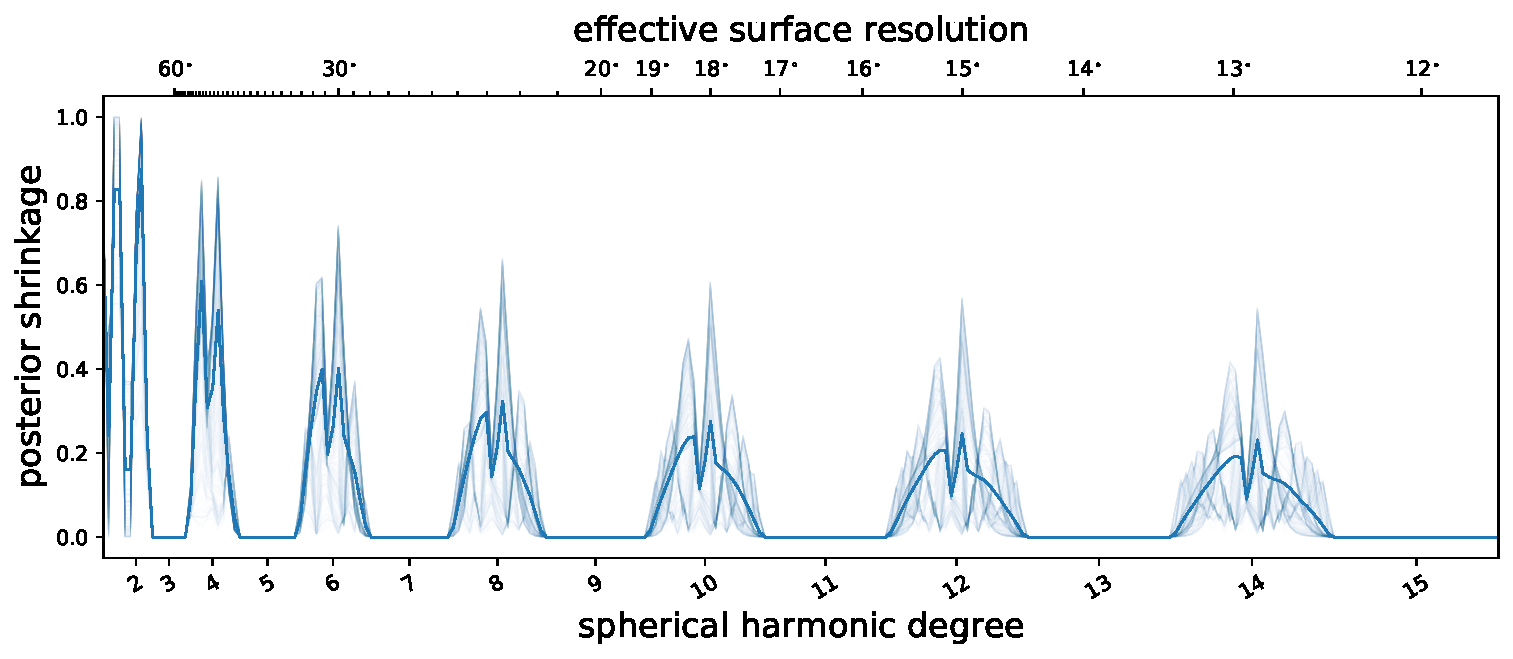
\includegraphics[width=\linewidth]{figures/nullspace_ensemble_single.pdf}
        \oscaption{nullspace_ensemble}{%
            Posterior shrinkage...
            \label{fig:nullspace_ensemble_single}
        }
    \end{centering}
\end{figure}

%
\begin{align}
    \label{eq:shrinkage}
    R \equiv 1 - \lim\limits_{\sigma_0^2 \rightarrow \infty}
    \frac{\sigma^2}{\sigma_0^2}
    \quad,
\end{align}
%

But what if the star rotates about a different axis? A useful property of
the spherical harmonics is that rotation about any axis can only change the
order $m$ of the harmonic, while keeping the degree $l$ fixed: in other
words, rotation simply mixes the spherical harmonics along rows in
Figure~\ref{fig:ylms}. Therefore, if we rotate the spherical harmonics
in the figure about a different axis, we are still subject to just as
many degeneracies (i.e., the size of the null space is unchanged),
but the particular linear combination of modes in the null space will
be different.

This all seems quite hopeless, and for analyses of individual stars,
it pretty much is. Unless extremely strong (and likely incorrect) priors are employed
(such as assuming the stellar surface consists of exactly two perfectly
circular, uniform contrast spots), we simply cannot learn much about
the surface of an individual star from photometry.

However, we can use the dependence of the null space on inclination to our
advantage. If we could observe a star from many different vantage points,
we would be able to break many of the degeneracies at play, since we
would get different constraints on the amplitude of each mode when viewed
at different inclinations. This, of course, is not possible (at least not
yet!). But what we \emph{can} do is observe many similar stars, each viewed
at a different (random) inclination, and attempt to learn something about
the properties of the ensemble of stars as a whole. This is exactly
what we did in \S\ref{sec:calibration}, where we showed that this kind
of ensemble analyses is not only possible but can also be extremely
constraining of the spot properties at the population level. In the
following section, we explore the role of ensemble analyses in breaking
the degeneracies of the mapping problem in more detail.



\subsection{Ensemble analyses work}
\label{sec:ensemble}

To quantify the power of ensemble analyses,
let us define the \emph{posterior shrinkage} $R$ for a given
spherical harmonic coefficient as
%
\begin{align}
    \label{eq:shrinkage}
    R \equiv 1 - \lim\limits_{\sigma_0^2 \rightarrow \infty}
    \frac{\sigma^2}{\sigma_0^2}
    \quad,
\end{align}
%
where $\sigma_0^2$ is the prior variance
and $\sigma^2$ is the posterior variance.
The posterior shrinkage is a measure of how informative a measurement is about a
given mode on the surface in the limit of infinite signal-to-noise ratio (SNR)
and is independent of what the stellar surface actually looks like.
If, at infinite SNR and with a completely uninformative prior,
a particular mode can be learned exactly from a dataset, the posterior
shrinkage is defined to be unity. Conversely, if the data is completely
unconstraining of that mode (i.e., it is entirely in the null space),
$R$ will tend to zero.

\begin{figure}[t!]
    \begin{centering}
        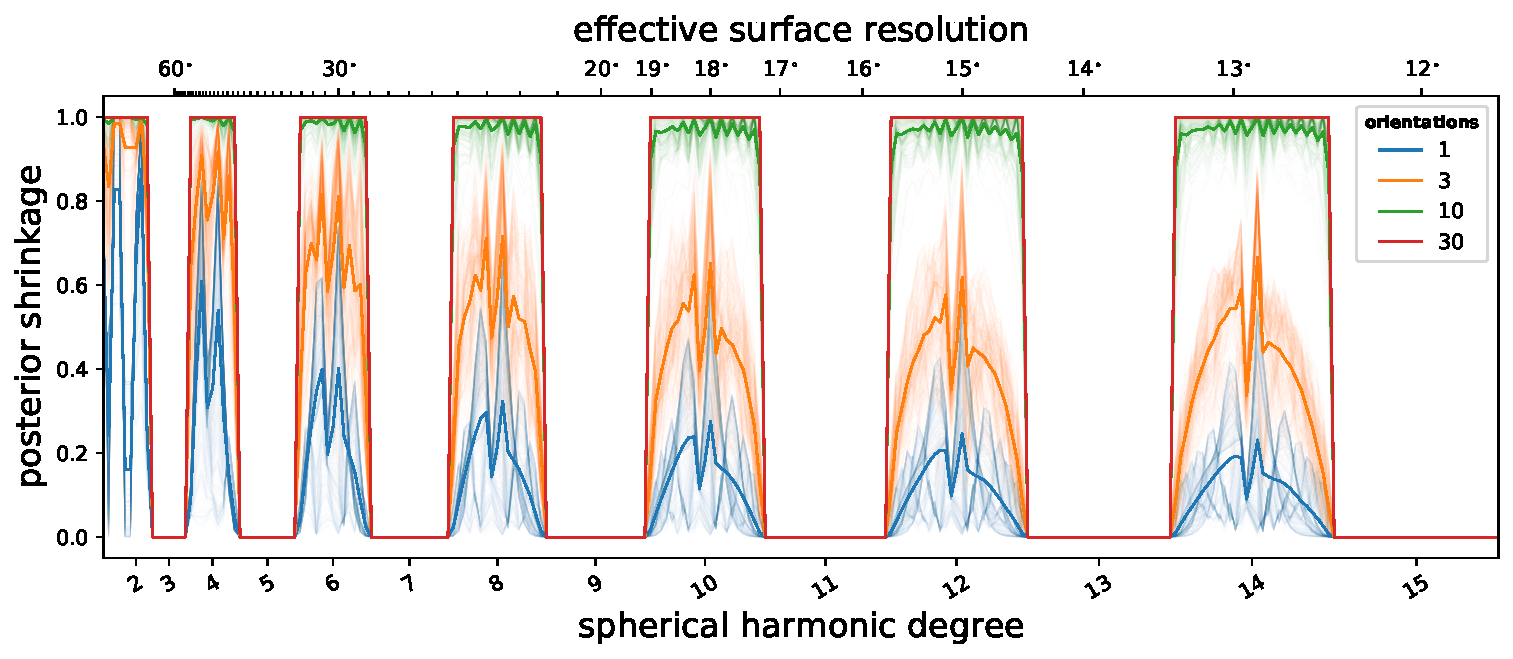
\includegraphics[width=\linewidth]{figures/nullspace_ensemble.pdf}
        \oscaption{nullspace_ensemble}{%
            Posterior shrinkage as a function of spherical harmonic degree
            for a hypothetical scenario in which an observer can measure the light curves
            of 1 (blue), 3 (orange), 10 (green), and 30 (red) \emph{identical} stars
            viewed at random orientations.
            The thicker curves correspond to
            the mean shrinkage for each experiment.
            The information content in the light curve of a star observed
            from a single vantage point approaches zero as $l$
            increases. However, observing many identical stars from different vantage points
            allows one to recover nearly all of the information in the
            even spherical harmonic modes. This is why ensemble analyses of
            many similar stars at different inclinations allows us to infer
            their surface properties.
            \label{fig:nullspace_ensemble}
        }
    \end{centering}
\end{figure}

Figure~\ref{fig:nullspace_ensemble} shows the posterior shrinkage
as a function of spherical harmonic degree for a few different hypothetical
scenarios in which we observe one or more stellar light curves with
no limb darkening.
Let us first consider the blue curves, in which a light curve is
collected from a single star viewed at a single random inclination (which, of course, is
all we can do from our fixed vantage point on Earth).
Each thin blue curve corresponds to a particular random draw from the (isotropic)
inclination distribution; the thick blue curve is the average over 300 trials.
For some of the low-degree modes, the shrinkage is relatively high: it is
fairly easy to constrain the dipole moment from a light curve, as this is
usually the dominant sinusoidal signal. However, as the degree $l$
increases, the shrinkage decreases dramatically: at $l = 14$, corresponding
to features on scales of roughly $15^\circ$, the light curve
can only tell us about $\sim 10\%$ of the total information about what the
surface looks like. As $l$ increases further, $R$ tends to zero.
Another important feature of the shrinkage, which we hinted at above,
is that it is exactly zero for
all odd-degree modes above $l = 1$. This is a well-known fact: all odd spherical
harmonics other than the dipole are in the null space \emph{regardless of
    inclination} \citep[e.g.,][]{Luger2019}. In other words, these spherical
harmonics are perfectly antisymmetric in projection over the unit disk
when viewed from any orientation. Absent structure to break these symmetries
(see below), we simply cannot learn anything about these modes from
stellar light curves. If we average over the shrinkage for all modes up to $l=15$,
we find that a single light curve measurement can only tell us $\sim 9\%$
of the information about the surface on those scales.

In an ensemble analysis, we assume we observe the lightcurves of many stars
that are ``similar'' in some statistical sense. As a thought experiment,
let us consider an extreme version of ensemble analysis in which all the
stars in our dataset happen to have \emph{identical} surfaces. We will
still assume they are oriented at random inclinations, as we would expect for
field stars. The orange curves in the top panel of the figure correspond to
the case in which we analyze ensembles consisting of three identical stars
viewed at three different random inclinations.
Interestingly, the shrinkage increased at all even spherical harmonic degrees
(the odd degrees, as we mentioned above, are always invisible).
Note that since we are in the limit of infinite SNR, the fact that we have
three times the data as we did in the previous scenario is irrelevant: the
increase in the shrinkage is instead due to the fact that our observations
from different vantage points broke some degeneracies in the problem.
This is a consequence of the fact we mentioned in the previous section:
the null space (for the even modes)
is a strong function of the inclination.
If we average over all modes, we obtain a total shrinkage of $\sim 24\%$
for $l\leq15$ in this case.

Finally, the green and red curves correspond respectively to ensembles of ten and thirty
identical stars observed at random inclinations.
In these scenarios, the posterior shrinkage
is nearly $100\%$
for all even modes (it asymptotically approaches $100\%$ as the number
of light curves increases further). The total shrinkage is $\sim 47\%$
and approaches $50\%$ as both $l_\mathrm{max}$  and the number of light curves
tend to infinity. Thus, if we were able to measure light curves of identical stars
from many different inclinations, the null space would consist \emph{only}
of the odd modes, and our data would tell us exactly half of all the
information about the surfaces of these objects.

\begin{figure}[t!]
    \begin{centering}
        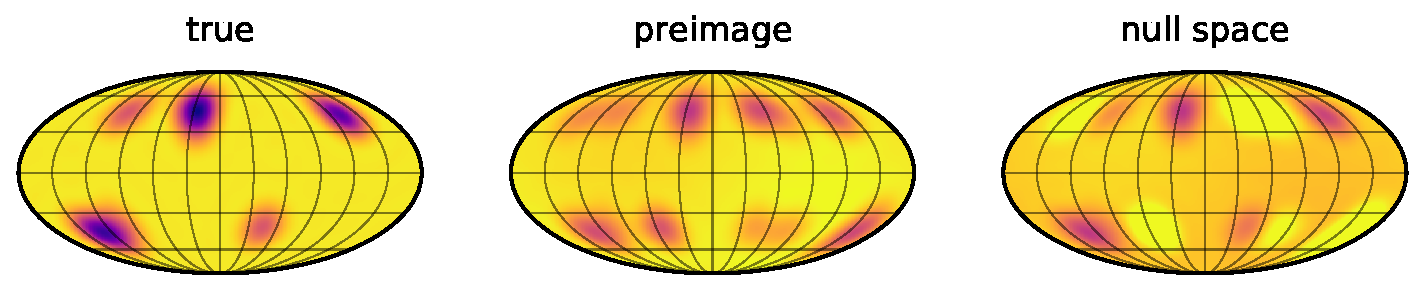
\includegraphics[width=\linewidth]{figures/evenmodes.pdf}
        \oscaption{evenmodes}{%
            A spotted stellar surface seen in Mollweide projection
            (left), the same surface with all odd $l > 2$ harmonics
            set to zero (center), and the same surface with $l = 1$
            and all even harmonics set to zero (right). The plot
            on the right represents the portion of the surface that is
            in the null space of the light curve problem at all
            inclinations; the plot in the center is the portion of the
            surface that can be inferred by combining observations
            made from all possible inclinations.
            \label{fig:evenmodes}
        }
    \end{centering}
\end{figure}

Figure~\ref{fig:evenmodes} shows a spotted stellar surface decomposed
into its \emph{preimage} and its \emph{null space} in the limiting case
in which its light curve can be observed at a large number of inclinations.
The former is the set of all modes that map onto the light curve (i.e.,
the complement of the null space). Because spots are compact features, they
are necessarily made up of a continuum of spherical harmonic modes spanning
many different values of $l$: they can therefore be seen in both the even
modes (the preimage) and the odd modes (the null space). Interestingly,
the symmetries at play require spots to be paired with antipodal dark mirror
images in the even modes, and with \emph{bright} ones in the odd modes
(which sum to perfectly cancel out in the true map). Since these reflections
are at the same latitude (in the opposite hemisphere) as the true spots,
they do not contribute any bias to our inference, which already assumes the
latitude distribution is symmetric about the equator. Thus, even though
we are only sensitive to the even modes in ensemble analyses, they are
sufficient to learn about the properties we are interested in.

In practice, the fact that stars are not identical complicates this picture.
We can still learn about the \emph{distribution} of spot properties, but
in general our ensemble must consist of far more light curves in order to
place strong constraints on these properties. As we showed in \S\ref{sec:calibration},
under ideal conditions an ensemble of $M = 50$ similar stars may be sufficient,
but in practice we may need on the order of hundreds or even a thousand light curves
in order to mitigate the effects of variance in the sample.

\subsection{Limb darkening}
\label{sec:limbdark}

\begin{figure}[t!]
    \begin{centering}
        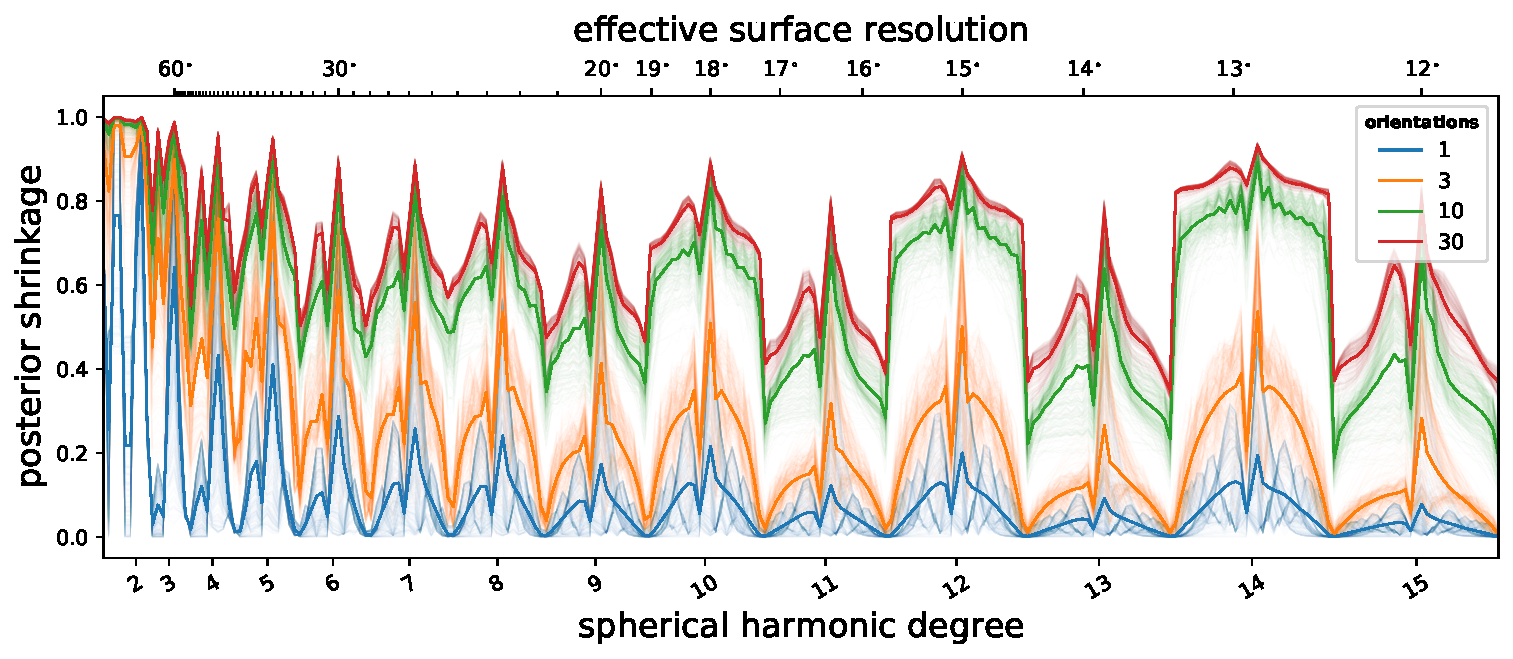
\includegraphics[width=\linewidth]{figures/nullspace_ensemble_ld.pdf}
        \\
        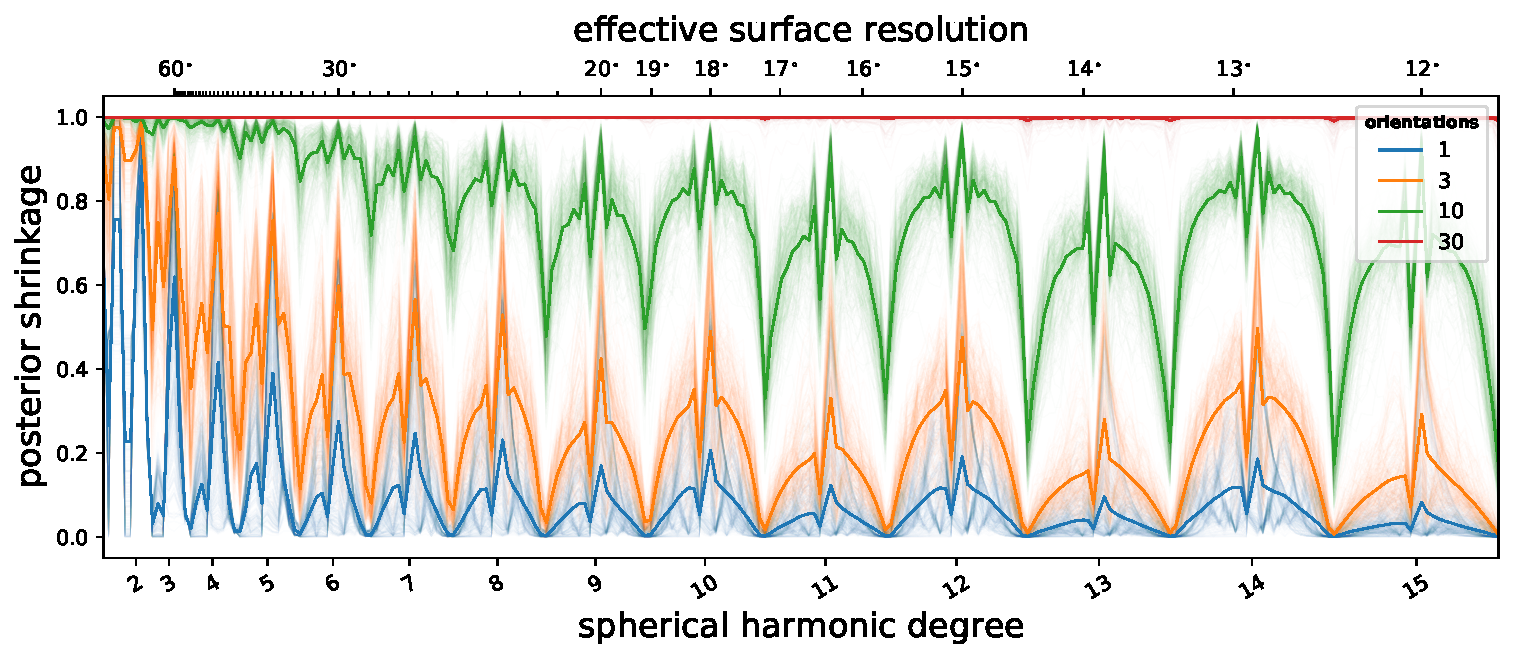
\includegraphics[width=\linewidth]{figures/nullspace_ensemble_ld_var.pdf}
        \oscaption{nullspace_ensemble_ld}{%
            \emph{Top:} Same as Figure~\ref{fig:nullspace_ensemble},
            but for limb-darkened
            stars with quadratic coefficients $u_1 = 0.5$ and $u_2 = 0.25$. Odd
            modes can now be probed, at the expense of the even modes.
            \emph{Bottom:} Same as the top panel, but allowing for
            a 10\% variation in $u_1$ and $u_2$
            across different observations. For $\gtrsim 30$ light curves,
            there is virtually no null space up to at least $l_\mathrm{max} = 15$.
            \codelink{nullspace_ensemble_ld_var}
            \label{fig:nullspace_ensemble_ld}
        }
    \end{centering}
\end{figure}

As we saw in Figure~\ref{fig:calibration_ld}, the presence of limb darkening
makes it significantly more difficult to infer spot properties at fixed
SNR. To understand
why, let us repeat the experiment from the previous section,
this time with moderate quadratic limb darkening ($u_1 = 0.5$ and $u_2 = 0.25$).
The top panel of Figure~\ref{fig:nullspace_ensemble_ld} shows the
posterior shrinkage plot (same as Figure~\ref{fig:nullspace_ensemble}, but
with limb darkening). Interestingly, there is no longer a clean division of
the null space between even and odd modes in the limit of large $M$.
This is because limb darkening effectively lifts odd modes out of the null space, \emph{at the
    expense of the even modes}. While no coefficient lies entirely in the
null space ($R = 0$) when limb darkening is present, no coefficient
can be uniquely inferred ($R = 1$), either. This can be understood by noting that
a polynomial limb darkening law can be written
exactly as a linear combination of the $m=0$ spherical harmonics
up to a degree equal to the order of the limb darkening
\citep[in this case, $l = 2$;][and Appendix~\ref{sec:ld}]{Luger2019,Agol2020}.
Since the limb darkening operation is a (multiplicative) downweighting of
the surface intensity, the map seen by the observer is just the product
of the spherical harmonic representation of the surface ($\mathbf{f}$)
and the spherical harmonic representation of the limb darkening profile.
And since spherical harmonics are just polynomials on the surface of the sphere,
the product of spherical harmonics of degree $l_1$ and $l_2$ is a spherical
harmonic of degree $l_1 + l_2$. This means that the linear limb darkening
component ($l = 1$) effectively raises the degree of all spherical harmonic
coefficients of the surface map by one. This has the effect of reversing
the null space: under \emph{only} linear limb darkening, it is the \emph{even}
modes that would like in the null space. However, the quadratic
limb darkening term ($l = 2$) raises the degree of all spherical harmonics by two,
so its presence ensures that the even modes can still be probed to some extent.
In reality, the true limb darkening profile of a stellar surface is more
complicated than a two-parameter quadratic model can capture; but one may still
expand it as an arbitrary order polynomial, in which case the argument still
applies---limb darkening mixes the null space and the preimage in a nontrivial
way. The fact that no coefficient can be determined uniquely---i.e., there are
perfect degeneracies involving \emph{all} modes on the surface---is what makes it more
difficult in practice to perform ensemble analyses on limb-darkened stars.
Nevertheless, it is still possible to uniquely and precisely infer the spot properties
under limb darkening,
but as a rule of thumb, the stronger the limb darkening, the larger the
ensemble must be (see Figure~\ref{fig:calibration_ld_1000}).

In reality, it is unlikely that all stars in a given ensemble have exactly
the same limb darkening coefficients, however ``similar'' the stars may be.
The bottom panel of Figure~\ref{fig:nullspace_ensemble_ld} shows the same
posterior shrinkage plot, but for the case where each star has coefficients
$u_1 = 0.5 \pm 0.05$ and $u_2 = 0.25 \pm 0.025$; i.e., we add a scatter of
10\% in the value of these coefficients. The plot shows the posterior
shrinkage in the hypothetical case where we know the coefficients for
each star exactly. Now, as the size of the ensemble increases, the posterior
shrinkage approaches unity \emph{for all spherical harmonic modes}.
In the same way that the null space is a strong function of the inclination,
allowing us to chip away at it with observations at different inclinations,
the null space is also a strong function of the limb darkening law. Even a
small amount of variance in the coefficients is sufficient to constrain all surface
modes exactly (in the limit of infinite SNR and large $M$).

In practice, of course, we will never know the limb darkening coefficients
exactly, so we must either model them or marginalize over them
(see \S\ref{sec:other-marg}). This will dilute our ability to infer surface
properties exactly.

\section{The baseline problem}
\label{sec:baseline}

There is one final subtle---but extremely important---point that remains to
be discussed in our derivation of a Gaussian process for stellar
rotation. Thus far we have cast the light curve problem in a typical GP inference
setting: we model our observations $\mathbbb{f}$ as
a multidimensional random variable distributed as a multivariate Gaussian with mean vector
$\pmb{\mu}$ and covariance matrix $\pmb{\Sigma}$. However, in the context of
relative photometry, the mean $\pmb{\mu}$ is typically \emph{unobservable}.
%
To understand why, consider what
$\pmb{\mu}(P, \mathbf{u}, \pmb{\theta}_\bullet)$ actually represents:
it is the expected value
of the flux,
\emph{in units of the flux one would measure if the star had no spots}.
We do not observe in these units: rather, we observe in units of counts on
the detector, which depend on the luminosity of the star, the distance to
the star, and various properties of the telescope. Even if we knew all these
things, we would still need to know the intrinsic photospheric brightness
in order to properly normalize our dataset for direct application of
the Gaussian process.

Instead, what astronomers typically do is to self-normalize their data:
i.e., divide the flux by the mean, median, maximum, or some similar
statistic of the light curve. This operation folds the unknowability of
the flux baseline under the rug and transforms the light curve into a \emph{relative}
measurement of the star's temporal variability. While relative measurements
are typically what we are interested in anyways, this normalization procedure
has two significant drawbacks: (1) it introduces a new set of perfect degeneracies
in the modeling and (2) it can substantially change the covariance structure
of the dataset.

The first point is illustrated in the toy example in
Figure~\ref{fig:mean_normalization}. As it has been pointed out before
\citep[e.g.,][]{Basri2018},
we will not spend too much time discussing it, other than to say that the
flux normalization introduces a degeneracy between the total spot coverage
of a star and the contrast of any individual feature on the surface.
The two stars in the figure have different numbers of spots, different
spot contrasts, and different total spot coverage. In ``absolute'' units, in which
the flux is measured as a fraction of the flux of an unspotted star, the two
light curves are distinct (top panel). However, we can only measure these light
curves up to an unknown multiplicative factor. Normalizing these light curves
to the ``continuum'' level yields the curves in the bottom panel, which are
\emph{perfectly} indistinguishable from each other. Normalization to the mean,
median, or any other statistic of the light curve does not help break this
degeneracy, which is inherent to relative photometry. While one could instead \emph{fit}
for the normalization as a latent variable, there is no information in the data
that can help break it, so the result will be entirely determined by the prior.%
\footnote{%
    In principle, the maximum level of a light curve could set a lower limit on
    the location of the baseline. However, this applies only if the surface is
    known to be made up of \emph{exclusively} dark spots. The presence of bright
    spots (faculae), which are common on the Sun, make it effectively impossible
    for one to infer the baseline from single-band relative photometry alone.
}
We discuss these issues further in \S\ref{sec:breaking_baseline_degeneracy}.

\begin{figure}[t!]
    \begin{centering}
        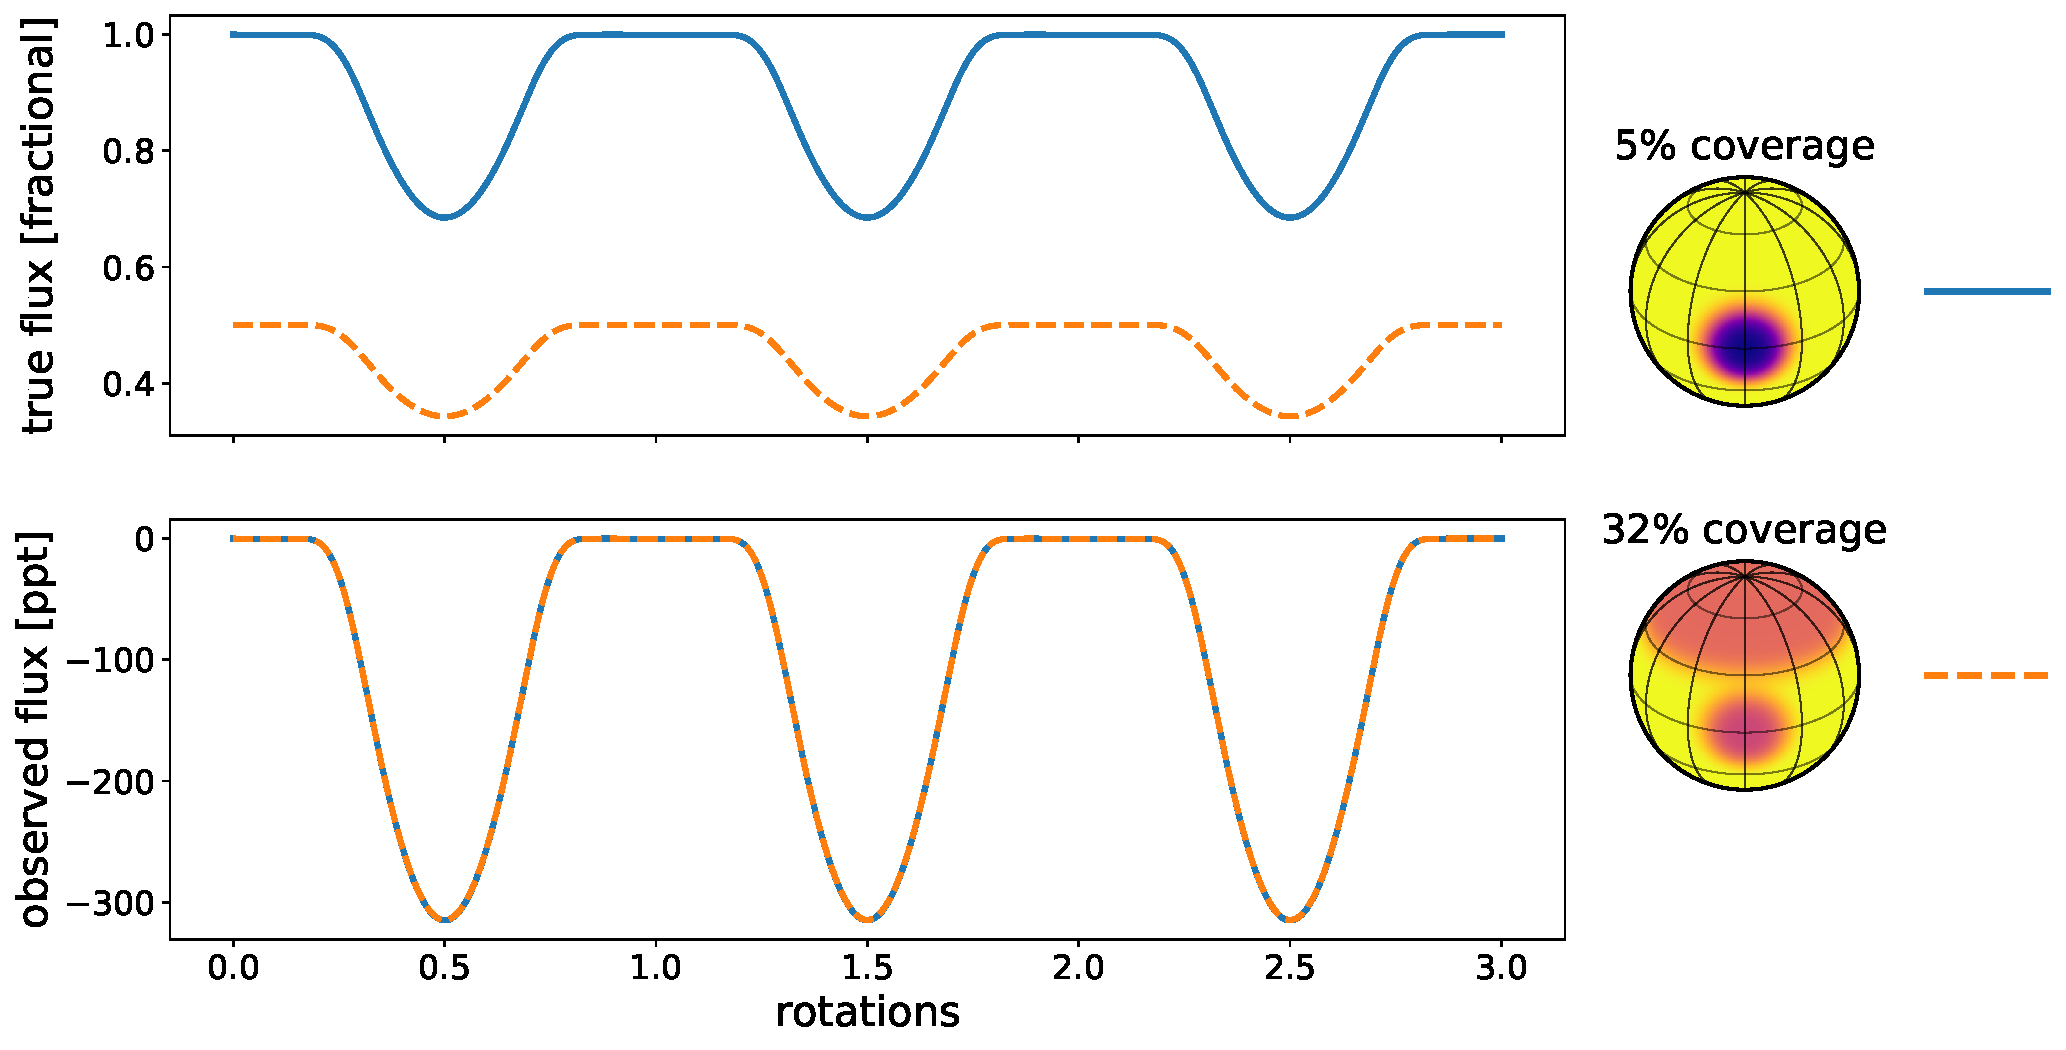
\includegraphics[width=\linewidth]{figures/mean_normalization.pdf}
        \oscaption{mean_normalization}{%
            An example of the baseline problem.
            \emph{Top:} Consider a star with a single
            equatorial spot of contrast $c$ viewed at a certain inclination.
            The total flux (in some units) as a function of time is shown as
            the blue curve. Now, consider a second star,
            identical in all respects to the first, except that (1) the equatorial spot
            has half the contrast (i.e., $\nicefrac{c}{2}$); and (2) there is
            a second, large spot centered on the pole. The corresponding light
            curve is shown as the dashed orange curve.
            The orange light curve is different from the blue one in two ways:
            (1) since the equatorial spot has half the contrast, the amplitude of the associated
            dips in the light curve is half that of the first star; and
            (2) since the polar spot is azimuthally symmetric, its only
            contribution is a net darkening at all phases.
            \emph{Bottom:} The true baseline level of a stellar
            light curve, which corresponds to the flux one would measure in the
            absence of any spots, is almost always unknown. Photometric measurements
            are therefore meaningful only in a relative sense, i.e., as deviations from
            the mean, median, or maximum level of the light curve.
            The bottom panel shows the same two light curves, this time plotted as
            deviations in parts per thousand (ppt) from their respective maxima.
            To the observer, the two light curves are \emph{indistinguishable}.
            In the absence of baseline information, there
            exists a perfect degeneracy between the total spot coverage
            and the contrast of any individual feature on the surface.
            As a consequence, the total spot coverage of a star cannot be
            inferred from relative photometry.
            \label{fig:mean_normalization}
        }
    \end{centering}
\end{figure}

The second point is of more immediate concern, since we must correct our
expression for the covariance matrix
$\pmb{\Sigma}(P, \mathbf{u}, \pmb{\theta}_\bullet)$ if we are to
use our GP to model normalized light curves. For definiteness, let us
consider only mean-normalized light curves.%
\footnote{In practice, the expressions derived below also work well
    for median-normalized light curves, since the distribution of the GP sample median
    is usually close to the distribution of the sample mean.}
Since we are dividing the
flux by the mean, one might imagine that we could simply divide the
covariance matrix by the square of the mean. However,
this is incorrect, since we must be careful to distinguish between the
\emph{sample} mean and the \emph{process} mean. When normalizing a light
curve by the mean, the operation we perform is
%
\begin{align}
    \label{eq:ftilde}
    \tilde{\mathbbb{f}\hspace{0.2em}} & = \frac{\mathbbb{f}}{\left<\mathbb{f}\right>}
    \quad,
\end{align}
%
where $\tilde{\mathbbb{f}\hspace{0.2em}}$ is the normalized, unit-mean light curve,
$\mathbbb{f}$ is the measured light curve (in detector counts), and
$\left<\mathbb{f}\right>$ is the \emph{sample} mean: i.e., the average value of
a given star's light curve (which we model as a sample from our GP).
This may be close to but is in general different from the \emph{process} mean,
$\pmb{\mu}(P, \mathbf{u}, \pmb{\theta}_\bullet)$, since the mean of
a draw from the GP is itself normally distributed with a variance that scales
with the GP variance.%
\footnote{
    Importantly, the sample mean and process mean will be different even in the
    absence of measurement error! In other words, the mean flux of a given
    star (i.e., the sample mean)
    will in general be different from the mean flux \emph{across all stars} with similar
    surface properties (the process mean).
}

Computing the covariance of the normalized process is tricky, especially
because the normalized process is \emph{not} strictly Gaussian: the distribution
has heavy tails due to the fact that $\tilde{\mathbbb{f}\hspace{0.2em}}$ diverges as
the sample mean approaches zero. In fact, because of these tails, the covariance
of the normalized process is formally \emph{infinite}, since the probability of
drawing a sample whose mean is arbitrarily close to zero is finite.

If this is all starting to sound like a bad idea, that's because it is!
A much safer approach is to resist the temptation to normalize the light curve
and instead model the unknown multiplicative amplitude as a latent variable. However,
this would require an extra parameter \emph{for every light curve}, so the
computational savings we achieved by marginalizing out the inclination
would be gone. Fortunately, in practice, the variance of a stellar light curve
is usually small compared to its mean: stellar variability amplitudes are
typically at the level of a few percent or lower. When this is the case,
the probability of drawing a GP sample whose mean is close to zero is
extremely small, and we can make use of the approximate expression derived
in \citet{Luger2021} for the covariance of a normalized Gaussian process:
%
\begin{proof}{test_normgp}
    \label{eq:SigmaTilde}
    \tilde{\pmb{\Sigma}}
    & \approx
    \frac{A}{\mu^2} \pmb{\Sigma} +
    z \Big(
    (A + B) \, (\mathbf{1} - \mathbf{q}) \, (\mathbf{1} - \mathbf{q})^\top
    - A \, \mathbf{q} \, \mathbf{q}^\top
    \Big)
    \quad,
\end{proof}
%
where
%
\begin{align}
    \label{eq:z}
    z & \equiv \frac{\left< \Sigma \right>}{\mu^2}
\end{align}
%
is the ratio of the average element in $\pmb{\Sigma}$
to the square of the mean of the Gaussian process,
$\mathbf{q}$ is the ratio of the average of each row in $\pmb{\Sigma}$
to the average element in $\pmb{\Sigma}$, and $A$, $B$ are
order unity and zero scalars, respectively,
given by the optimally-truncated diverging series
%
\begin{align}
    \label{eq:baseline_alpha}
    A
     & \equiv
    \sum\limits_{i=0}^{i_\mathrm{max}}
    \frac{(2i + 1)!}{2^i \, i!}
    z^i
    \\[1em]
    \label{eq:baseline_beta}
    B
     & \equiv
    \sum\limits_{i=0}^{i_\mathrm{max}}
    \frac{2i(2i + 1)!}{2^i \, i!}
    z^i
    \quad,
\end{align}
%
where $i_\mathrm{max}$ is the largest value for which the series coefficient at $i_\mathrm{max}$ is
smaller than the coefficient at $i_\mathrm{max} - 1$. In the expressions above, it is
assumed that the mean $\pmb{\mu}$ is constant, i.e., $\pmb{\mu} = \mu\, \mathbf{1}$.
Since our Gaussian process is azimuthally isotropic (i.e., no preferred
longitude), that is the case throughout this paper.

What Equation~(\ref{eq:SigmaTilde}) allows us to do is effectively marginalize over
the unknown baseline by modeling the \emph{normalized} flux as a draw
from a Gaussian process:
%
\begin{align}
    \tilde{\mathbbb{f}\hspace{0.2em}}
    \left(P, \mathbf{u}, \pmb{\theta}_\bullet\right)
    \sim
    \mathcal{N}\left(
    \mathbf{1},
    \tilde{\pmb{\Sigma}} \left(P, \mathbf{u}, \pmb{\theta}_\bullet\right)
    \right)
    \quad.
\end{align}
%
This is appropriate as long as $z \ll 1$, for which the true
distribution of $\tilde{\mathbbb{f}\hspace{0.2em}}$ is approximately Gaussian. In practice,
we recommend employing this trick only for $z \lesssim 0.02$, for which the
error in the approximation to the covariance is less than $10^{-6}$.
In cases where the light curve variability exceeds about ten percent, we recommend
modeling the multiplicative amplitude in each light curve as a latent variable, as discussed
above.

\begin{figure}[p!]
    \begin{centering}
        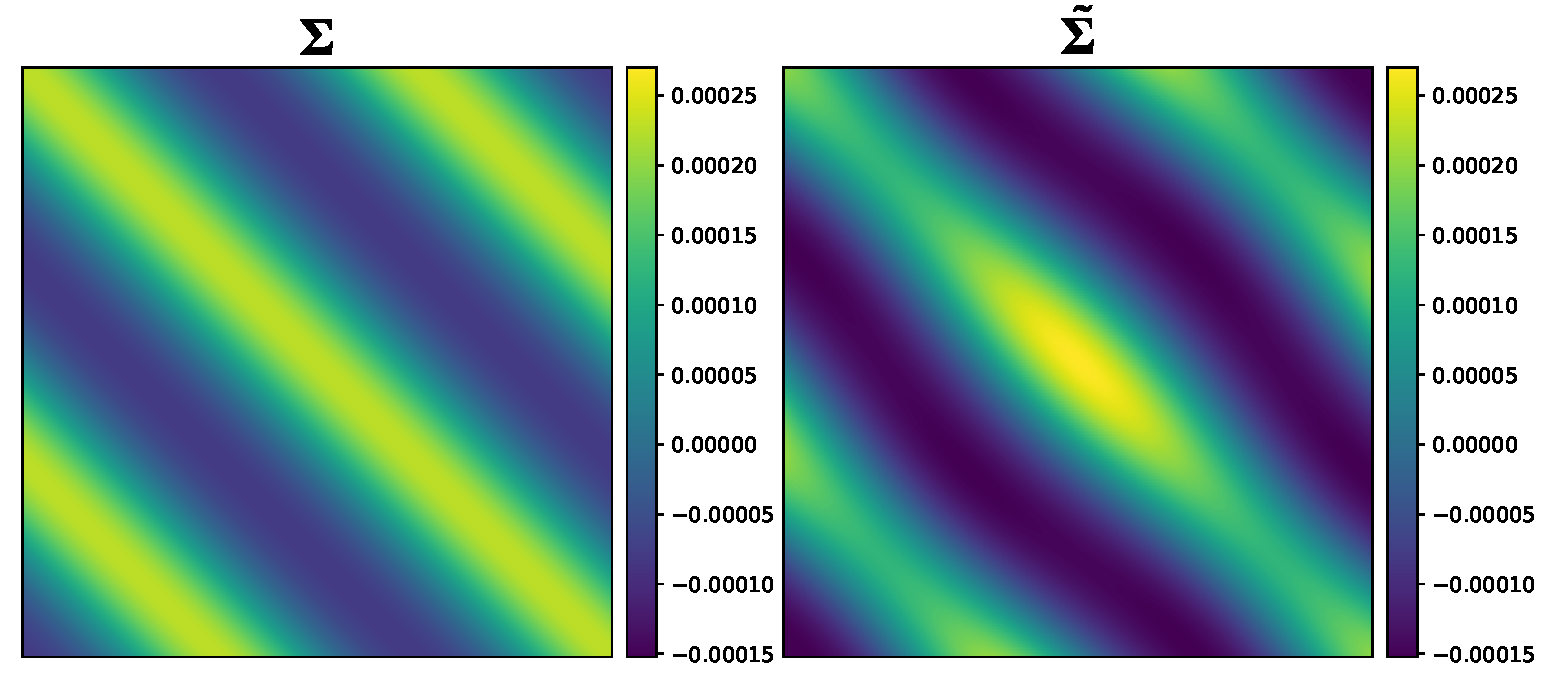
\includegraphics[width=\linewidth]{figures/normgp.pdf}
        \oscaption{normgp}{%
            An example of a flux covariance matrix $\pmb{\Sigma}$ for a
            \starry process (left) and the corresponding covariance of the
            normalized process (right), computed from Equation~(\ref{eq:SigmaTilde}).
            In addition to an offset and an overall scaling relative to the
            original covariance matrix, the covariance of the normalized process
            is discernibly non-stationary (see Figure~\ref{fig:nonstationarity}).
            \label{fig:normgp}
        }
    \end{centering}
\end{figure}

\begin{figure}[p!]
    \begin{centering}
        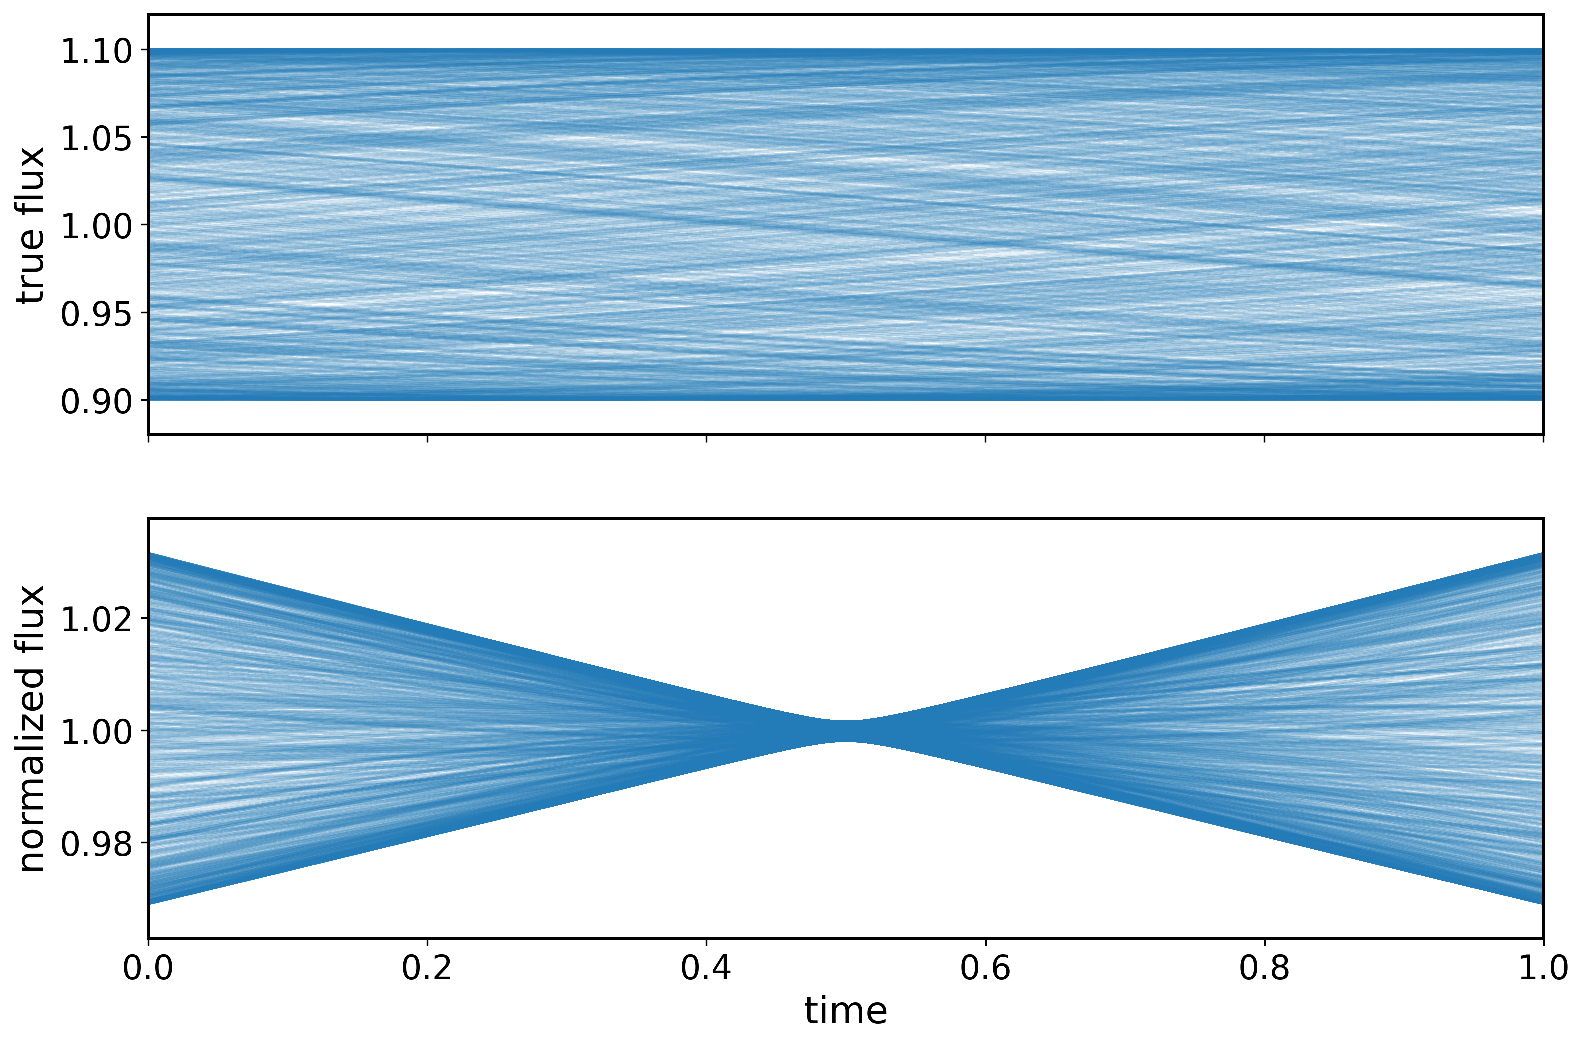
\includegraphics[width=\linewidth]{figures/nonstationarity.pdf}
        \oscaption{nonstationarity}{%
            An example of why normalized light curves are non-stationary.
            The top panel shows $1{,}000$ samples from a unit-mean sinusoid with
            an amplitude of 10\% and a period of 10 days, much longer than the
            1 day observation baseline. The bottom panel shows the same light curves,
            each normalized to its own mean. Because the mean tends to be near
            the center of the observation window, points near $t=0.5$ are driven
            to values very close to unity, while points near the edges have much
            larger scatter.
            \label{fig:nonstationarity}
        }
    \end{centering}
\end{figure}

Figure~\ref{fig:normgp} shows an example of a covariance matrix normalized
according to the procedure outlined above. The principal difference between
the normalized covariance and the original covariance is an overall
scaling and a small offset. However, the normalization also results in
the process becoming non-stationary: the covariance between two points in
a light curve is now slightly dependent on their phases.

To understand why normalized light curves are non-stationary, it is useful to
consider the
toy example in Figure~\ref{fig:nonstationarity}, in which we draw
$1{,}000$ samples from a sinusoid with period ten times longer than the
observational baseline. In this limit, each light curve is approximately
linear, which causes its mean value to roughly coincide with the midpoint of the
observation window. Division by the mean value results in points near the
midpoint being driven to unity and points near the edges (whose values differ
the most from the mean) to be driven to both large and small values. The
variance across all samples is now distinctly phase-dependent.
%
In general, the non-stationarity will be most extreme in cases where the
observation window is shorter than or comparable to one period, and
asymptotically vanishes in the limit that a large number of cycles are
observed.

\subsection{The baseline degeneracy}
\label{sec:breaking_baseline_degeneracy}

We showed in \S\ref{sec:calibration-inference} that in relative photometry there exists a
strong degeneracy between the contrast of individual spots $c$ and
the total number of spots $n$ on a star. Inspection of the
dependence of the GP on $c$ and $n$ (c.f. Appendix~\ref{sec:integrals}) reveals
that the mean and variance of the GP scale as
%
\begin{align}
    \mu      & = 1 - c \, n \, g (I, \mathbf{u}, r, \mu_\phi, \sigma_\phi)
    \nonumber                                                              \\
    \sigma^2 & = c^2 \, n \, h (I, \mathbf{u}, r, \mu_\phi, \sigma_\phi)
    \quad,
\end{align}
%
for some function $g$ and some function $h$ of the inclination,
the limb darkening coefficients, the spot radius, and the spot latitude
parameters.
If our observations were sensitive to both the true mean and
variance of stellar light curves,
we could uniquely infer $c$ and $n$. However, as we discussed in \S\ref{sec:baseline},
to good approximation, relative photometry can only tell us about the \emph{ratio}
%
\begin{align}
    \frac{\sigma^2}{\mu^2}
     & \propto \frac{c^2 n}{(1 - c n g)^2}
    \quad,
\end{align}
%
where $g$ is a complicated function of the (unknown) stellar and spot parameters;
relative photometry cannot tell us about the values of $c$ and $n$ independently.

The reason for this is that the relationship between the amplitude of the
light curve (measured in, e.g., counts per second on the detector)
and the fractional intensity deficit due to spots on the surface of
the star is not known. It is easy enough to normalize a light curve to its
mean, median, or maximum to obtain what we typically refer to as
``fractional'' or ``relative'' units, but this is \emph{not the same
    thing}! Consider the two stellar surfaces in Figure~\ref{fig:mean_normalization},
whose true light curves---measured in units where an unspotted star would
have unit flux---have different baselines and different amplitudes (top panel).
This is not what we observe when we do photometry---instead, we observe these
light curves multiplied by an unknown amplitude, which depends on (potentially
knowable) factors such as the luminosity of the star, the distance to it,
and the efficiency of the detector but also on the (typically unknowable)
unspotted photospheric brightness, which sets the true baseline level.
%
Division of these light curves by their (observed) baseline levels
(which is the operation typically done on stellar light curves) yields the
``relative'' light curves in the bottom panel, which are \emph{indistinguishable}
from each other. In this example, we are unable to distinguish between
models of the surface with different spot contrasts and number of spots (as well
as total spot ``coverage''). In general, these quantities cannot be learned
from single-band photometric measurements.
%

A direct consequence of the baseline degeneracy is that it is not in general
possible to constrain the total spot coverage of a star from relative,
single-band photometry. Assuming no spot overlap, the total spot coverage $f_S$ is simply the (average) area of a spot
times the total number of spots divided by the total area of the sphere, which
may be expressed as
%
\begin{proof}{test_fS}
    \label{eq:fS}
    f_S = \frac{1}{2}\left(1 - \left<\cos r\right>\right)n
    \quad,
\end{proof}
%
recalling that $r$ is the \emph{angular} radius of the spot.
While $r$ may be constrained from the covariance structure of the data
(\S\ref{sec:calibration-inference}), $n$ cannot.

The arguments above are based on the \emph{Gaussian approximation} to the
distribution of stellar light curves. As we discussed in \S\ref{sec:why-calibrate},
the true distribution has higher order moments that we do not consider here.
It is possible in principle that these moments could encode information to
break the $c-N$ degeneracy, but these are in general much more difficult
to constrain from the data. And even if this were the case, the fact remains
that degeneracies like the polar spot effect are fundamental: recall
Figure~\ref{fig:mean_normalization}, in which the two stars
have identical relative light curves, but very different spot coverage
fractions.

Fortunately, it may be possible to break these degeneracies (at least to some extent)
by collecting photometric data in multiple wavelength bands, an idea that has
been explored recently \citep[e.g.,][]{Gully2017,Guo2018}. Assuming the
locations and sizes of a star's spots are constant in wavelength, the amplitude
of the light curve in different bands (and in particular its slope as a function
of wavelength) can be used to directly constrain the
temperature, and hence the contrast, of the spots. This effectively breaks the
$c-N$ degeneracy. In practice, the effective size of spots may be different
at different wavelengths, which could complicate this picture somewhat. An extension
of the formalism in this paper to multi-band photometry, and a detailed investigation
of the information content of such observations, is left to future work.

\bibliography{bib}

\end{document}
